\documentclass[aspectratio=169]{beamer}

\usecolortheme[RGB={08,164,255}]{structure}
\usetheme[height=8mm]{Rochester}
\setbeamertemplate{items}[ball]
\setbeamertemplate{blocks}[rounded][shadow=true]
\setbeamertemplate{navigation symbols}{}
\usefonttheme{structurebold}
\usepackage[english]{babel}
\usepackage{lmodern}
\usepackage{makeidx}
\usepackage{amsmath}
\usepackage{amsfonts}
\usepackage{graphicx}
\usepackage{rotating} 
\usepackage[intoc]{nomencl} 
\usepackage{amssymb} 
\usepackage{pgfpages}
\usepackage{overpic}
\usepackage{subcaption}
\usepackage{nicefrac}
\usepackage{color, colortbl}
\usepackage{empheq}
\usepackage{tcolorbox}
\usepackage{dsfont}
\usepackage{mathtools,cancel,multicol}
%\usepackage{caption}
%\captionsetup[figure]{labelformat=empty}
\captionsetup[table]{labelformat=empty}
\usepackage{float,tikz,pgfplotstable}
\usetikzlibrary{positioning}
\usetikzlibrary{fit}
% ... (rest of your preamble continues unchanged) ...
\usepackage{xstring}
\usetikzlibrary{decorations.markings}
\usetikzlibrary{shapes.arrows}
\usepgfplotslibrary{fillbetween}
\newlength{\stabfreqwidth}
\newlength{\stabboundwidth}
\newlength{\stabestimlwidth}
\newlength{\stabestimmwidth}
\setlength{\stabfreqwidth}{5cm}
\setlength{\stabboundwidth}{2pt}
\setlength{\stabestimmwidth}{2pt}
\setlength{\stabestimlwidth}{1pt}
%%%%%%%
\usepackage{pgfplots}
\usepackage{tikz-3dplot} %after pgfpages and pgfplots
\usetikzlibrary{decorations.text}
\pgfplotsset{compat=newest}
\usepgfplotslibrary{colorbrewer}
\usetikzlibrary[patterns]
\usetikzlibrary{arrows,positioning,shapes}  
\usetikzlibrary{plotmarks}
\usetikzlibrary{decorations.pathmorphing}
\usetikzlibrary{calc}

\usepgfplotslibrary{statistics}

\tikzset{
    myarrow/.style={
        draw,
        fill=red,
        single arrow,
        minimum height=4.5ex,
        single arrow head extend=1ex
    }
}
\newcommand{\arrowup}{%
\tikz [baseline=-0.5ex]{\node [myarrow,rotate=90] {};}
}
\newcommand{\arrowdown}{%
\tikz [baseline=-1ex]{\node [myarrow,rotate=-90] {};}
}
\newcommand{\arrowright}{%
\tikz [baseline=-1ex]{\node [myarrow,rotate=0] {};}
}
\usepackage{pifont}
\newcommand{\tickYes}{\textcolor{green!80!blue!}{\ding{51}}}%
\newcommand{\tickNo}{\textcolor{red}{\ding{55}}}%

\newcommand*{\TakeFourierOrnament}[1]{{%
\fontencoding{U}\fontfamily{futs}\selectfont\char#1}}
\newcommand*{\danger}{\textcolor{red}{\TakeFourierOrnament{66}}}

\newlength{\plotwidth}
\newlength{\plotheight}

\newlength{\subplotwidth}
\newlength{\subplotheight}

\newlength{\trisubplotwidth}
\newlength{\trisubplotheight}

%\setlength{\plotwidth}{8cm}
 \setlength{\plotwidth}{0.9\textwidth}
%\setlength{\plotheight}{7cm}
\setlength{\plotheight}{0.85\textheight}

\setlength{\subplotwidth}{0.45\textwidth}
\setlength{\subplotheight}{\textwidth}

\setlength{\trisubplotwidth}{0.3\textwidth}
\setlength{\trisubplotheight}{0.3\textwidth}
%
%
\setbeamertemplate{footline}{%
   \raisebox{5pt}{\makebox[\paperwidth]{\hfill\makebox[10pt]{\tiny\insertframenumber}}}}
%%%% ARROW
\usetikzlibrary{fadings,shapes.arrows,shadows}  
\tikzfading[name=arrowfading, top color=transparent!0, bottom color=transparent!95]
\tikzset{arrowfill/.style={top color=blue!20, bottom color=blue!70, general shadow={fill=black, shadow yshift=-0.8ex, path fading=arrowfading}}}
\tikzset{arrowstyle/.style={draw=blue,arrowfill, single arrow,minimum height=#1, single arrow,
single arrow head extend=.4cm,}}
\newcommand{\tikzfancyarrow}[2][2cm]{\tikz[baseline=-0.5ex]\node [arrowstyle=#1] {#2};}
% Custom commands
\newcommand{\ds}{\displaystyle}
\newcommand{\bs}{\boldsymbol}
\newcommand{\wt}{\widetilde}
\newcommand{\wtb}[1]{\overline{\widetilde{#1}}} 
\newcommand{\wtbF}[1]{\overline{\widetilde{\bsF}}} 
\newcommand{\ol}{\overline}
\newcommand{\tcr}{\textcolor{red}}
\newcommand{\tcw}{\textcolor{white}}
\newcommand{\tcb}{\textcolor{blue}}
\newcommand{\tcc}{\textcolor{cyan}}
\newcommand{\bsmu}{\boldsymbol{\mu}}
\newcommand{\sig}{\sigma}
\newcommand{\bssig}{\boldsymbol{\sigma}}
\newcommand{\bsrho}{\boldsymbol{\rho}}
\newcommand{\eps}{\varepsilon}
\newcommand{\bseps}{\boldsymbol{\varepsilon}}
\newcommand{\bsk}{\boldsymbol{k}}
\newcommand{\bsx}{\boldsymbol{x}}
\newcommand{\bsF}{\boldsymbol{F}}
\newcommand{\bsE}{\boldsymbol{E}}
\newcommand{\bsH}{\boldsymbol{H}}
\newcommand{\bsJ}{\boldsymbol{J}}
\newcommand{\bsM}{\boldsymbol{M}}
\newcommand{\bsnabla}{\boldsymbol{\nabla}}
\newcommand{\dO}{d\Omega}
\newcommand{\p}{\mathfrak{p}}
\newcommand{\f}{\mathfrak{f}}
\newcommand{\Crossred}{$\mathbin{\tikz [x=1.4ex,y=1.4ex,line width=.2ex, red] \draw (0,0) -- (1,1) (0,1) -- (1,0);}$}% 
\newcommand{\Crossblue}{$\mathbin{\tikz [x=1.4ex,y=1.4ex,line width=.2ex, blue] \draw (0,0) -- (1,1) (0,1) -- (1,0);}$}% 
\renewcommand\u{\mathbf{u}}
\newcommand\bv{\mathbf{v}}
\newcommand\g{\mathbf{g}}
\newcommand\e{{\mbox{\boldmath $\varepsilon$}}}
\newcommand\bsi{{\mbox{\boldmath $\sigma$}}}
\newcommand\C{\mathcal{C}}
\newcommand\bdiv{{\mathbf{div}}}
\newcommand\R{\mathbb{R}}
\newcommand\bze{{\mbox{\boldmath $\zeta$}}}
\newcommand\I{\mathbf{I}}
\newcommand\tr{\mathrm{tr}}

\DeclareMathOperator*{\argmin}{arg\,min}

\newlength{\xmax}
\setbeamercovered{transparent}

\usepackage{multirow}

\definecolor{material1}{RGB}{243,217,24}
\definecolor{material2}{RGB}{0,101,19}
\definecolor{material3}{RGB}{59,59,248}
\definecolor{material4}{RGB}{0,225,94}
\definecolor{material5}{RGB}{0,170,255}
\definecolor{material1_3}{RGB}{0,255,223}
\definecolor{material2_3}{RGB}{0,191,255}
\definecolor{material3_3}{RGB}{59,59,248}
\definecolor{myGreen}{RGB}{46,139,87}
\definecolor{myblue}{RGB}{08,164,255}
\definecolor{jon_green}{rgb}{0.0, 0.5, 0.0}

\hypersetup{colorlinks,linkcolor=,urlcolor=myblue}
%this scales is necessary to scale a tikz to textwith
\usepackage{environ}
\newsavebox{\measure@tikzpicture}
\NewEnviron{scaletikzpicturetowidth}[1]{%
  \def\tikz@width{#1}%
  \def\tikzscale{1}\begin{lrbox}{\measure@tikzpicture}%
  \BODY
  \end{lrbox}%
  \pgfmathparse{#1/\wd\measure@tikzpicture}%
  \edef\tikzscale{\pgfmathresult}%
  \BODY
}

   \newif\ifdeveloppath
    \tikzset{/tikz/develop clipping path/.is if=developpath,
      /tikz/develop clipping path=true}

    \newcommand{\clippicture}[2]{
      \begin{tikzpicture}
    % Include the image to determine the size and set up the relative coordinate system. Enclose the \includegraphics in \phantom{} once the clipping path has been set up
    \ifdeveloppath
      \node[anchor=south west,inner sep=0] (image) at (0,0) {\includegraphics#1};
    \else
      \node[anchor=south west,inner sep=0] (image) at (0,0) {\phantom{\includegraphics#1}};
    \fi
    \pgfresetboundingbox
    \begin{scope}[x={(image.south east)},y={(image.north west)}]
      % Draw grid while developing clipping path
      \ifdeveloppath
        \draw[help lines,xstep=.1,ystep=.1] (0,0) grid (1,1);
        \foreach \x in {0,1,...,9} { \node [anchor=north] at (\x/10,0) {0.\x}; }
        \foreach \y in {0,1,...,9} { \node [anchor=east] at (0,\y/10) {0.\y}; }
        \draw[red, ultra thick] #2 -- cycle;
      \else
        % Use the path to clip, include the image
        \path[clip] #2 -- cycle;
        \node[anchor=south west,inner sep=0pt] {\includegraphics#1};
      \fi
    \end{scope}
    \end{tikzpicture}
    }
%make blocks with variable color    
\newenvironment{variableblock}[3]{%
  \setbeamercolor{block body}{#2}
  \setbeamercolor{block title}{#3}
  \begin{block}{#1}}{\end{block}}

%to put transparency in image
\usepackage{transparent}
%to create \mybullet{1}{text}
\newcommand{\mybullet}[2]{
\begin{tikzpicture}
\node (A) at (0,0){};
\shade [shading=ball, ball color=structure]  (A) circle (.2);
\node at (0,0){\small \textbf{\textcolor{white}{#1}}};
\node [right=0.2cm of A]{\large #2};
\end{tikzpicture}
}    
% Carlos Tikz preamble
\usetikzlibrary{arrows,positioning} 
\tikzset{
    %Define standard arrow tip
    >=stealth',
    %Define style for boxes
    punkt/.style={
           rectangle,
           rounded corners,
           draw=black, very thick,
           text width=4em,
           minimum height=2em,
           text centered},
    % Define arrow style
    pil/.style={
           ->,
           thick,
           shorten <=2pt,
           shorten >=2pt,}
}

\tikzset{
  invisible/.style={opacity=0},
  visible on/.style={alt={#1{}{invisible}}},
  alt/.code args={<#1>#2#3}{%
    \alt<#1>{\pgfkeysalso{#2}}{\pgfkeysalso{#3}} % \pgfkeysalso doesn't change the path
  },
}

\newcommand{\roundpic}[4][]{
  \tikz\node [circle, minimum width = #2,
    path picture = {
      \node [#1] at (path picture bounding box.center) {
        \includegraphics[width=#3]{#4}};
    }] {};}
    
\usepackage[ruled, vlined]{algorithm2e}
\SetKwComment{Comment}{/* }{ */}
\SetKwInput{KwOutput}{Output}

\usepackage{booktabs, multirow}
\newlength{\plotwidthmesh}
\setlength{\plotwidthmesh}{0.49\textwidth}
\newcommand{\subplotwidthhp}{0.49\textwidth}

\renewcommand{\H}{\mathbb{H}} % H: Hilbert Spaces
\newcommand{\abs}[1]{\left|#1\right|}
\newcommand{\norm}[1]{\left\|#1\right\|}
\newcommand{\te}{\tilde{\epsilon}}
\newcommand{\calT}{\mathcal{T}}
\newcommand{\grad}{\nabla}
\newcommand{\scalar}[2]{\left<#1\,,#2\right>}
\newcommand{\scalaire}[2]{\left<#1\,,#2\right>}
\newcommand{\m}{\mathbf{m}}
\newcommand{\x}{\mathbf{x}}
\newcommand{\M}{\mathbf{M}}
\newcommand{\umi}{u_{\mathbf{m}_i}}

\title{Easy-to-implement $hp$-adaptivity for \\ non-elliptic goal-oriented problems}
\author{ Felipe Vinicio Caro Gutiérrez\inst{2,1} \\
\vspace{0.3cm}
\small \textcolor{myblue}{\hspace{-0.0cm} \textit{Supervisors:}}  David Pardo\inst{1,2,3}, Elisabete Alberdi\inst{1}
}
%\bigskip
\institute{\inst{1} \footnotesize University of the Basque Country (UPV/EHU), Bilbao, Spain
 \and \vspace{-0.2cm} \inst{2}  \footnotesize  Basque Center for Applied Mathematics (BCAM), Bilbao, Spain
  \and \vspace{-0.2cm} \inst{3} \footnotesize Ikerbasque, Bilbao, Spain }
%\date{\includegraphics[height=0.35\textheight]{./figures/M2OP_V.png}}
%
\date{  29 November 2023, Leioa
}

\setbeamercolor{author}{fg=black!80!white}
\setbeamercolor{date}{fg=black!80!white}
\setbeamercolor{institute}{fg=black!70!white}
\setbeamerfont*{date}{family=\sffamily,series=\bf,size=\scriptsize}
\setbeamerfont*{title}{family=\sffamily,series=\bf,size=\large}
\setbeamerfont*{author}{family=\sffamily,series=\bfseries,size=\large}
\setbeamerfont*{institute}{family=\sffamily,series=\bf,size=\small}
  
% !TEX spellcheck = English
\newcommand*{\PbName}{}
\newcommand*{\GOAPbName}{}
\newcommand*{\EnergyPbName}{}
\newcommand*{\ColName}{}
\newcommand*{\FigurePath}{Figures}
\newcommand*{\DataPath}{}
%
%\tikzset{/tikz/external/export next=false}
%
% ==========
% \directadjointsolution
% ==========
\newcommand*{\directadjointsolution}[5]{%
  \renewcommand*{\DataPath}{\FigurePath/#1}
  \pgfplotsset{%
    colormap={paraview}{rgb=(0.231373, 0.298039, 0.752941) rgb=(0.865003, 0.865003, 0.865003) rgb=(0.705882, 0.0156863, 0.14902)}%
  }%
  \pgfplotsset{colormap name={paraview}}%

  \getelemdbl{\DataPath/#3_#2_ColorbarValues.dat}{min_value}{0}{\scaleMin}
  \getelemdbl{\DataPath/#3_#2_ColorbarValues.dat}{max_value}{0}{\scaleMax}
  \getelemdbl{\DataPath/#3_#2_ColorbarValues.dat}{mean_value}{0}{\scaleMean}

  \begin{tikzpicture}
    \begin{axis}[name=master,
        width=\textwidth,height=\textwidth,
        enlargelimits=false,
        xlabel=$x$,
        ylabel=$y$,
        xlabel near ticks,
        ylabel near ticks,
        colorbar horizontal,
        colorbar style={%
            xtick={\scaleMin,\scaleMean,\scaleMax},
            title={#4 solution},
            at={(master.above north west)},anchor=south west,
            yshift=0.5em,
            title style={
                yshift=2pt
            },
            xticklabel pos=upper,
        },
        point meta min=\scaleMin,
        point meta max=\scaleMax,
        xmin=0, xmax=1,
        ymin=0, ymax=1,
        xtick={0,0.5,1},
        ytick={0,0.5,1},
        tick align=outside,
        axis y line*=#5, % Position of y axis, left or right
        axis x line*=bottom,
        axis line style={draw=none},
        tick style={draw=none},
    ]
      \addplot [forget plot] graphics[xmin=0,xmax=1,ymin=0,ymax=1] {\DataPath/coarse_mesh_fine_#2_#3.png};
    \end{axis}
  \end{tikzpicture}
}
% ==========
% \goasolutions
% ==========
\newcommand*{\goasolutions}[2]{%
  \renewcommand*{\DataPath}{\FigurePath/#1/hp/order_1}
  \findmax{\DataPath/outputs.txt}{iter}{\endIter}

  \FormatIntegerTwoDigit{\endIter}{\endIterformated}
  \FormatIntegerThreeDigit{\endIter}{\endIterformatedthree}
  %
  \begin{subfigure}[t]{0.4\textwidth}
    \centering
    \directadjointsolution{#1/hp/order_1}{\endIterformated}{Direct_solution_#2}{Direct}{left}%
    \caption{Solution to the direct problem.}
    \label{fig:#1_dir}
  \end{subfigure}
  ~
  \begin{subfigure}[t]{0.4\textwidth}
   \centering
   \directadjointsolution{#1/hp/order_1}{\endIterformated}{Adjoint_solution_#2}{Adjoint}{right}%
    \caption{Solution to the adjoint problem.}
    \label{fig:#1_adj}
  \end{subfigure}
}
% ==========
% \plothpmeshes
% ==========
\newcommand{\plothpmeshes}[2][]{
  \renewcommand{\DataPath}{\FigurePath/#2/hp/order_1}
  \findmax{\DataPath/outputs.txt}{iter}{\endIter}
  \FormatIntegerTwoDigit{\endIter}{\endIterformated}
  \FormatIntegerThreeDigit{\endIter}{\endIterformatedthree}

  \only<+>{%
    \begin{figure}
      \centering
      \foreach \i in {x,y}{%
        \begin{subfigure}[t]{0.4\textwidth}
          \centering
          \hpmeshes{#2/hp/order_1}{\endIterformatedthree}{\i}%
          \subcaption{Final $hp$-adapted mesh with polynomial orders in the \i-direction.} 
        \end{subfigure}
      }
      %\caption{Final $hp$-adapted meshes after the adaptivity}
    \end{figure}
  }
}
% ========
% \hpmeshes
% ========
\newcommand{\hpmeshes}[3]{%
  \renewcommand{\DataPath}{\FigurePath/#1}

  \lastelement{\DataPath/outputs.txt}{MaxP}{\maxp}
  \lastelement{\DataPath/outputs.txt}{MinP}{\minp}
  \pgfplotsset{colormap/YlOrRd}
  \begin{tikzpicture}
    \begin{axis}[name=master,
        width=\textwidth,height=\textwidth,
        enlargelimits=false,
        xlabel=$x$,
        ylabel=$y$,
        xlabel near ticks,
        ylabel near ticks,
        axis line style={draw=none},
        tick style={draw=none},
        hide axis,
        colorbar horizontal,
        colorbar style={%
            xtick={1,3,...,\maxp},
            title={Order of approximation},
            at={(master.above north west)},anchor=south west,
            yshift=1em,
            title style={
                yshift=2pt
              },
            xticklabel pos=upper,
          },
        point meta min=1,
        point meta max=\maxp,
      ]
      %
      \ifstrequal{#1}{}{%
        \addplot [forget plot] graphics[xmin=-1,xmax=1,ymin=-1,ymax=1] {\DataPath/mesh_#3_#2.png};
      }{%
        \addplot [forget plot] graphics[xmin=0,xmax=1,ymin=0,ymax=1] {\DataPath/mesh_#3_#2.png};
      }
    \end{axis}
  \end{tikzpicture}
}
% ==========
%\comparerrors
% ==========
\newcommand{\comparerrors}[2][]{
  \begin{subfigure}[t]{0.48\textwidth}
    \centering
    \errorleft[#2]{Lower}
  \end{subfigure}
   ~
 \begin{subfigure}[t]{0.48\textwidth}
    \centering
    \errorright[#2]{Error}
  \end{subfigure}
}
% ======
%\errorleft
% ======
\newcommand{\errorleft}[2][]{
  \renewcommand{\DataPath}{\FigurePath/#1}
  \renewcommand{\PbName}{#1} 
  \renewcommand{\ColName}{#2}

  \begin{tikzpicture}
    \pgfplotsset{xmode=log}

    \begin{axis}[name=mainerrorplot,
        xlabel={nDoFs (log scale)},
        ylabel=Relative error in \% (log scale),
        ymode=log,
        xmode=log,
        width=\textwidth,height=\plotheight,
        ylabel near ticks,
        xlabel near ticks,
        enlargelimits=true,
        legend style={draw=black,fill=white,legend cell align=left, at={(0.5,1.01)}, anchor=south},
        legend columns=-1
      ]
        %
        % Plot for hp
	\pgfplotstableread{\FigurePath/\PbName/hp/order_1/outputs.txt}\loadedtable
	\addplot+[line width=1pt] table[x expr=\thisrow{nr_dof}, y expr=\thisrow{\ColName}] {\loadedtable}
	node[pos=0.75, pin={[pin edge=solid, pin distance=0.4cm]270:$hp$}] {}; 

	% Plot for h with p=1
	\pgfplotstableread{\FigurePath/\PbName/h/order_1/outputs.txt}\loadedtable
	\addplot+[line width=1pt] table[x expr=\thisrow{nr_dof}, y expr=\thisrow{\ColName}] {\loadedtable}
	node[pos=0.8, pin={[pin edge=solid, pin distance=0.5cm]90:$h$ ($p=1$)}] {};

	% Plot for h with p=2
	\pgfplotstableread{\FigurePath/\PbName/h/order_2/outputs.txt}\loadedtable
	\addplot+[line width=1pt] table[x expr=\thisrow{nr_dof}, y expr=\thisrow{\ColName}] {\loadedtable}
	node[pos=0.05, pin={[pin edge=solid, pin distance=0.4cm]0:$h$ ($p=2$)}] {};
     
    \end{axis}
  \end{tikzpicture}
   {\caption{Evolution of $\tilde{e}_{\textrm{rel}}^{\textrm{\, energy}}$ in the process.}}
}
% =======
%\errorright
% =======
\newcommand{\errorright}[2][]{
  \renewcommand{\DataPath}{\FigurePath/#1}
  \renewcommand{\PbName}{#1} 
  \renewcommand{\ColName}{#2}

  \begin{tikzpicture}
    \pgfplotsset{xmode=log}

    \begin{axis}[name=mainerrorplot,
        xlabel={nDoFs (log scale)},
        ymode=log,
        xmode=log,
        yticklabel pos=right,
        width=\textwidth,height=\plotheight,
        ylabel near ticks,
        xlabel near ticks,
        enlargelimits=true,
        legend style={draw=black,fill=white,legend cell align=left, at={(0.5,1.01)}, anchor=south},
        legend columns=-1
      ]
      %
      % Plot for hp
\pgfplotstableread{\FigurePath/\PbName/hp/order_1/outputs.txt}\loadedtable
\addplot+[line width=1pt] table[x expr=\thisrow{nr_dof}, y expr=\thisrow{\ColName}] {\loadedtable}
node[pos=0.95, pin={[pin edge=solid, pin distance=0.4cm]90:$hp$}] {}; 

% Plot for h with p=1
\pgfplotstableread{\FigurePath/\PbName/h/order_1/outputs.txt}\loadedtable
\addplot+[line width=1pt] table[x expr=\thisrow{nr_dof}, y expr=\thisrow{\ColName}] {\loadedtable}
node[pos=0.5, pin={[pin edge=solid, pin distance=0.1cm]90:$h$ ($p=1$)}] {};

% Plot for h with p=2
\pgfplotstableread{\FigurePath/\PbName/h/order_2/outputs.txt}\loadedtable
\addplot+[line width=1pt] table[x expr=\thisrow{nr_dof}, y expr=\thisrow{\ColName}] {\loadedtable}
node[pos=0.1, pin={[pin edge=solid, pin distance=0.4cm]270:$h$ ($p=2$)}] {};


    \end{axis}
  \end{tikzpicture}
  {\caption{Evolution of $e_{\textrm{rel}}^{\textrm{QoI}}$ in the process.}}
}

\tikzset{mark size=3}
% =========
% \plothpunref
% =========
\newcommand{\plothpunref}[1]{
    \renewcommand{\DataPath}{\FigurePath/Unref/#1/hp/order_1}
    \findmax{\DataPath/outputs.txt}{iter}{\endIter}

    \findmax{\FigurePath/#1/hp/outputs.txt}{iter}{\endIterh}

    \FormatIntegerTwoDigit{\endIterh}{\endIterhformated}

    \begin{center}
        \begin{figure}
            \foreach \i in {1,2,...,\endIter}{%
                \only<+>{%
                    \begin{subfigure}{\subplotwidthhp}
                        \centering
                        \FormatIntegerThreeDigit{\i}{\iformat}
                        \plothpmeshunref{Unref/#1/hp/order_1}{\iformat}{#1/hp/coarse_mesh_fine_\endIterhformated_Direct_solution_abs} % custom command
                        \subcaption{Adaptive iteration \i ~of \endIter}
                    \end{subfigure}
                    \begin{subfigure}{\subplotwidthhp}
                        \centering
                        % % %
                        \errorplotlog{Unref/#1/hp/order_1}{\i} % custom command
                        \subcaption{ Evolution of the relative error}
                    \end{subfigure}
                    \only<1->{\caption{Adaptive process for a Helmholtz problem}}
                }%
            }
        \end{figure}
    \end{center}
}
% =============
% \plothpmeshunref
% =============
\newcommand{\plothpmeshunref}[3]{%
    \renewcommand{\DataPath}{\FigurePath/#1}

    \begin{tikzpicture}
        \begin{axis}[
            name=master,
            width=\textwidth,
            height=\textwidth,
            enlargelimits=false,
            xlabel=$x$,
            ylabel=$y$,
            xlabel near ticks,
            ylabel near ticks,
            hide axis,
        ]
        %

        \addplot [forget plot] graphics[xmin=0,xmax=1,ymin=0,ymax=1] {\DataPath/mesh_X_#2.png};
        \addplot [forget plot, opacity=0.2] graphics[xmin=0,xmax=1,ymin=0,ymax=1] {\FigurePath/#3};

        \end{axis}
    \end{tikzpicture}%
}

\pgfplotsset{select coords between index/.style 2 args={
    x filter/.code={
        \ifnum\coordindex<#1\def\pgfmathresult{}\fi
        \ifnum\coordindex>#2\def\pgfmathresult{}\fi
    }
}}
% =========
% \errorplotlog
% =========
\newcommand{\errorplotlog}[2]{
    \renewcommand{\DataPath}{\FigurePath/#1}

    \findmax{\DataPath/outputs.txt}{nr_dof}{\maxdof}
    \findmin{\DataPath/outputs.txt}{nr_dof}{\mindof}
    \findmaxDbl{\DataPath/outputs.txt}{Error}{\maxerror}
    \findminDbl{\DataPath/outputs.txt}{Error}{\minerror}

    \begin{tikzpicture}
        %\pgfplotsset{ log y ticks with fixed point,}
        \begin{axis}[
            name=mainerrorplot,
            xlabel={Number of DoF},
            ylabel=Relative error in the QoI (\%),
            ymode=log,
            xmode=log,
            ymin=1e-7,
            ymax=1e3,
            xmin=\mindof,
            xmax=\maxdof,
            width=0.9\textwidth,
            height=0.85\plotwidthmesh,
            ylabel near ticks,
            xlabel near ticks,
            enlargelimits=true,
            legend style={
                draw=black,
                fill=white,
                legend cell align=left,
                at={(0.5,1.01)},
                anchor=south
            },
            legend columns=-1
        ]

        \addplot+[
            line width=1pt,
            select coords between index={0}{#2}
        ] table[
            x expr=\thisrow{nr_dof},
            y expr=\thisrow{Error}
        ] {\FigurePath/#1/outputs.txt};

        \end{axis}
    \end{tikzpicture}
}
% ============
%\compareconver
% ============
\newcommand{\compareconver}[3][]{
  \begin{subfigure}[t]{0.48\textwidth}
    \centering
    \converleft[#1]{#2}{#3}{Error}
  \end{subfigure}
  ~
 \begin{subfigure}[t]{0.48\textwidth}
    \centering
    \converright[#1]{#2}{#3}{Lower}
  \end{subfigure}
}
% ========
%\converleft
% ========
\newcommand{\converleft}[4][]{
  \renewcommand{\DataPath}{\FigurePath/#2}
  \renewcommand{\GOAPbName}{#2} 
  \renewcommand{\EnergyPbName}{#3} 
  \renewcommand{\ColName}{#4}

  \begin{tikzpicture}
    \pgfplotsset{xmode=log}
    
    \begin{axis}[name=mainerrorplot,
          xlabel={Number of DoF},
          ylabel=Relative error in \% (log scale),
          ymode=log,
          xmode=log,
           width=\textwidth,height=\plotheight,
          ylabel near ticks,
          xlabel near ticks,
          enlargelimits=true,
          legend style={draw=black,fill=white,legend cell align=left, at={(0.5,1.01)}, anchor=south},
          legend columns=-1
        ]
        %
        \foreach\method in {#1}{												
          \ifthenelse{\equal{\method}{hp}}{
            \foreach \order in {1}{
                \edef\temp{\noexpand\addlegendentry{GOA}}
                \pgfplotstableread{\FigurePath/\GOAPbName/hp/order_\order/outputs.txt}\loadedtable
                \addplot+[ line width=1pt] table[x expr=\thisrow{nr_dof},y expr=\thisrow{\ColName}] {\loadedtable};
                \temp
                
                \edef\temp{\noexpand\addlegendentry{energy-norm}}
                \pgfplotstableread{\FigurePath/\EnergyPbName/hp/order_\order/outputs.txt}\loadedtable
                \addplot+[ line width=1pt] table[x expr=\thisrow{nr_dof},y expr=\thisrow{\ColName}] {\loadedtable};
                \temp
              }
          }{}
        }
      \end{axis}
  \end{tikzpicture}
  \caption{Evolution of goal-oriented adaptivity.}
  \label{subfig:compagoal}
}
% =========
%\converright
% =========
\newcommand{\converright}[4][]{
  \renewcommand{\DataPath}{\FigurePath/#2}
  \renewcommand{\GOAPbName}{#2} 
  \renewcommand{\EnergyPbName}{#3} 
  \renewcommand{\ColName}{#4}
  
  \begin{tikzpicture}
    \pgfplotsset{xmode=log}
    
    \begin{axis}[name=mainerrorplot,
          xlabel={Number of DoF},
          ymode=log,
          xmode=log,
          yticklabel pos=right,
          width=\textwidth,height=\plotheight,
          ylabel near ticks,
          xlabel near ticks,
          enlargelimits=true,
          legend style={draw=black,fill=white,legend cell align=left, at={(0.5,1.01)}, anchor=south},
          legend columns=-1
        ]
        %
 	\foreach\method in {#1}{												
          \ifthenelse{\equal{\method}{hp}}{
            \foreach \order in {1}{
                \edef\temp{\noexpand\addlegendentry{GOA}}
                \pgfplotstableread{\FigurePath/\GOAPbName/hp/order_\order/outputs.txt}\loadedtable
                \addplot+[ line width=1pt] table[x expr=\thisrow{nr_dof},y expr=\thisrow{\ColName}] {\loadedtable};
                \temp
                
                 \edef\temp{\noexpand\addlegendentry{energy-norm}}
                \pgfplotstableread{\FigurePath/\EnergyPbName/hp/order_\order/outputs.txt}\loadedtable
                \addplot+[ line width=1pt] table[x expr=\thisrow{nr_dof},y expr=\thisrow{\ColName}] {\loadedtable};
                \temp
              }
          }{}
        }
      \end{axis}
  \end{tikzpicture}
  \caption{Evolution of energy-norm adaptivity.}
  \label{subfig:compaenergy}
}
% =========
%\plotsolution
% =========
\newcommand{\plotsolution}[2][]{
  \renewcommand{\DataPath}{\FigurePath/#2/hp/order_1}
  \findmax{\DataPath/outputs.txt}{iter}{\endIter}

  \FormatIntegerTwoDigit{\endIter}{\endIterformated}
  \FormatIntegerThreeDigit{\endIter}{\endIterformatedthree}
  \begin{center}
  \begin{subfigure}[t]{0.425\textwidth}
  	\energysolution{#2/hp/order_1}{\endIterformated}{Direct_solution_real}{#1}%
	\caption{Solution of the example 1.}
  \end{subfigure}
  \end{center}
}
% ===========
%\energysolution
% ===========
\newcommand{\energysolution}[4]{
  \renewcommand{\DataPath}{\FigurePath/#1}
  
  \pgfplotsset{
      colormap={paraview}{rgb=(0.231373, 0.298039, 0.752941) rgb=(0.865003, 0.865003, 0.865003) rgb=(0.705882, 0.0156863, 0.14902)}%
    }
    \pgfplotsset{colormap name={paraview}}

    \getelemdbl{\DataPath/#3_#2_ColorbarValues.dat}{min_value}{0}{\scaleMin}
    \getelemdbl{\DataPath/#3_#2_ColorbarValues.dat}{max_value}{0}{\scaleMax}
    \getelemdbl{\DataPath/#3_#2_ColorbarValues.dat}{mean_value}{0}{\scaleMean}

    \begin{tikzpicture}
      \begin{axis}[name=master,
          width=\textwidth,height=\textwidth,
          enlargelimits=false,
          xlabel=$x$,
          ylabel=$y$,
          xlabel near ticks,
          ylabel near ticks,
          xtick={0,0.5,1},
          ytick={0,0.5,1},
          colorbar horizontal,
          colorbar style={
              xtick={\scaleMin,\scaleMean,\scaleMax},
              title={Value of the solution},
              at={(master.above north west)},anchor=south west,
              yshift=2pt,
              title style={
                  yshift=5pt
                },
              yshift=0.2em,
              xticklabel pos=upper,
            },
          point meta min=\scaleMin,
          point meta max=\scaleMax,
        ]
        \addplot [forget plot] graphics[xmin=0,xmax=1,ymin=0,ymax=1] {\DataPath/coarse_mesh_fine_#2_#3.png};
      \end{axis}
    \end{tikzpicture}
}
% ==========
%\plotmaterials
% ==========
\newcommand{\plotmaterials}[2][]{
  \renewcommand{\DataPath}{\FigurePath/#2/hp/order_1}
  \findmax{\DataPath/outputs.txt}{iter}{\endIter}

  \FormatIntegerTwoDigit{\endIter}{\endIterformated}
  \FormatIntegerThreeDigit{\endIter}{\endIterformatedthree}
  \begin{center}
  	\materials{#2/hp/order_1}{\endIterformated}{materials}{#1}%
  \end{center}
}
% =======
%\materials
% =======
\newcommand{\materials}[4]{
  \renewcommand{\DataPath}{\FigurePath/#1}

    \pgfplotsset{
      colormap={paraview}{rgb=(0.05, 1.0, 1.0) rgb=(1.0, 0.0, 0.0) rgb=(0.0, 1.0, 0.0) rgb=(0.0, 0.0, 1.0)}%
    }
    \pgfplotsset{colormap name={paraview}}%
    \findmax{\DataPath/#3.txt}{uno}{\matuno}
    \findmax{\DataPath/#3.txt}{dos}{\matdos}
    \findmax{\DataPath/#3.txt}{tres}{\mattres}
    \findmax{\DataPath/#3.txt}{cuatro}{\matcuatro}

    \begin{tikzpicture}
      \begin{axis}[name=master,
          width=\textwidth*0.5,height=\textwidth*0.5,
          enlargelimits=false,
          axis line style={draw=none},
          tick style={draw=none},
          xticklabels={},
          yticklabels={},
          colorbar horizontal,
          colorbar sampled,
          colormap access=piecewise constant,
          colorbar style={
              samples=4,
              xtick=data,
              xticklabels={0.01,1,10,1000},
              xticklabel style={xshift=\textwidth*0.5/10},
              title={Diffusivity of the materials},
              at={(master.above north west)},anchor=south west,
              yshift=5pt,
              title style={
                  yshift=5pt
                },
              yshift=0.2em,
              xticklabel pos=upper,
            },
        ]
        %
        \addplot [forget plot] graphics[xmin=0,xmax=1,ymin=0,ymax=1] {\DataPath/#3_#2.png};
      \end{axis}
    \end{tikzpicture}
}
%%%%%%%%%%%%%%%%%%%%%%%%%%%%%%%%%%%%%%%%%%%%%%%%%%%%%%%% OLD
% ==============
% elemental routines
% ==============
\newcommand{\FormatIntegerTwoDigit}[2]{
  \pgfmathsetbasenumberlength{2}
  \pgfmathbasetodec#2{#1}{10}
}

\newcommand{\FormatIntegerThreeDigit}[2]{
  \pgfmathsetbasenumberlength{3}
  \pgfmathbasetodec#2{#1}{10}
}

\newcommand{\getelem}[4]{
  \pgfplotstablegetelem{#3}{#2}\of{#1}%
  \pgfmathtruncatemacro#4{\pgfplotsretval}
  \pgfplotstableclear{\datatable}
}


\newcommand{\getelemdbl}[4]{
  \pgfplotstablegetelem{#3}{#2}\of{#1}%
  \pgfmathsetmacro#4{\pgfplotsretval}
  \pgfplotstableclear{\datatable}
}

\newcommand{\findmax}[3]{
  \pgfplotstableread{#1}{\datatable}
  \pgfplotstablesort[sort key={#2},sort cmp={float >}]{\sorted}{\datatable}%
  \pgfplotstablegetelem{0}{#2}\of{\sorted}%
  \pgfmathtruncatemacro#3{\pgfplotsretval}
  \pgfplotstableclear{\datatable}
}

\newcommand{\findmin}[3]{
  \pgfplotstableread{#1}{\datatable}
  \pgfplotstablesort[sort key={#2},sort cmp={float <}]{\sorted}{\datatable}%
  \pgfplotstablegetelem{0}{#2}\of{\sorted}%
  \pgfmathtruncatemacro#3{\pgfplotsretval}
  \pgfplotstableclear{\datatable}
}

\newcommand{\findmaxDbl}[3]{
  \pgfplotstableread{#1}{\datatable}
  \pgfplotstablesort[sort key={#2},sort cmp={float >}]{\sorted}{\datatable}%
  \pgfplotstablegetelem{0}{#2}\of{\sorted}%
  \pgfmathsetmacro#3{\pgfplotsretval}
  \pgfplotstableclear{\datatable}
}

\newcommand{\lastelement}[3]{
  \pgfplotstableread{#1}{\datatable}
  \pgfplotstablegetrowsof{\datatable} 
  \pgfmathtruncatemacro{\rows}{\pgfplotsretval}
  \pgfmathtruncatemacro{\lastrow}{\rows-1}
  \pgfplotstablegetelem{\lastrow}{#2}\of{\datatable}
  \pgfmathsetmacro#3{\pgfplotsretval}
  \let#3=\pgfplotsretval
  \pgfplotstableclear{\datatable}
}

\newcommand{\findminDbl}[3]{
  \pgfplotstableread{#1}{\datatable}
  \pgfplotstablesort[sort key={#2},sort cmp={float <}]{\sorted}{\datatable}%
  \pgfplotstablegetelem{0}{#2}\of{\sorted}%
  \pgfmathsetmacro#3{\pgfplotsretval}
  \let#3=\pgfplotsretval
  \pgfplotstableclear{\datatable}
}

\pgfplotsset{
  log x ticks with fixed point/.style={
      xticklabel={
          \pgfkeys{/pgf/fpu=true}
          \pgfmathparse{exp(\tick)}%
          \pgfmathprintnumber[fixed relative, precision=3]{\pgfmathresult}
          \pgfkeys{/pgf/fpu=false}
        }
    },
  log y ticks with fixed point/.style={
      yticklabel={
          \pgfkeys{/pgf/fpu=true}
          \pgfmathparse{exp(\tick)}%
          \pgfmathprintnumber[fixed relative, precision=3]{\pgfmathresult}
          \pgfkeys{/pgf/fpu=false}
        }
    }
}

\pgfplotscreateplotcyclelist{custom list style}{%
  color=red, solid, every mark/.append style={solid},mark size=4.0pt,mark=o\\%
  color=blue, solid, every mark/.append style={solid},mark size=3.0pt,mark=square\\%
  color=gray!20!black!40, solid, every mark/.append style={solid}, mark size=2.5pt, mark=triangle\\%
  color=black, solid, every mark/.append style={solid},mark=diamond*\\%
  color=black!50!red, solid, every mark/.append style={solid}, mark=otimes*\\%
  color=black!50!yellow, loosely dashed, every mark/.append style={solid},mark=*\\%
  color=black!50!blue,densely dashed, every mark/.append style={solid},mark=square*\\%
  color=black!50!magenta,dashdotted, every mark/.append style={solid},mark=otimes*\\%
  color=black!50!orange,dashdotdotted, every mark/.append style={solid},mark=star\\%
  color=black!50!cyan, densely dashdotted,every mark/.append style={solid},mark=diamond*\\%
}

\pgfplotsset{%
  every axis plot/.append style= {line width=2pt},
  cycle list name=custom list style,
}

%%%%%%%%%%%%%%%%%%%%%%%%%%%%%%%%%%
\begin{document}
{
\usebackgroundtemplate{\tikz\node[opacity=0.1,inner sep=0] {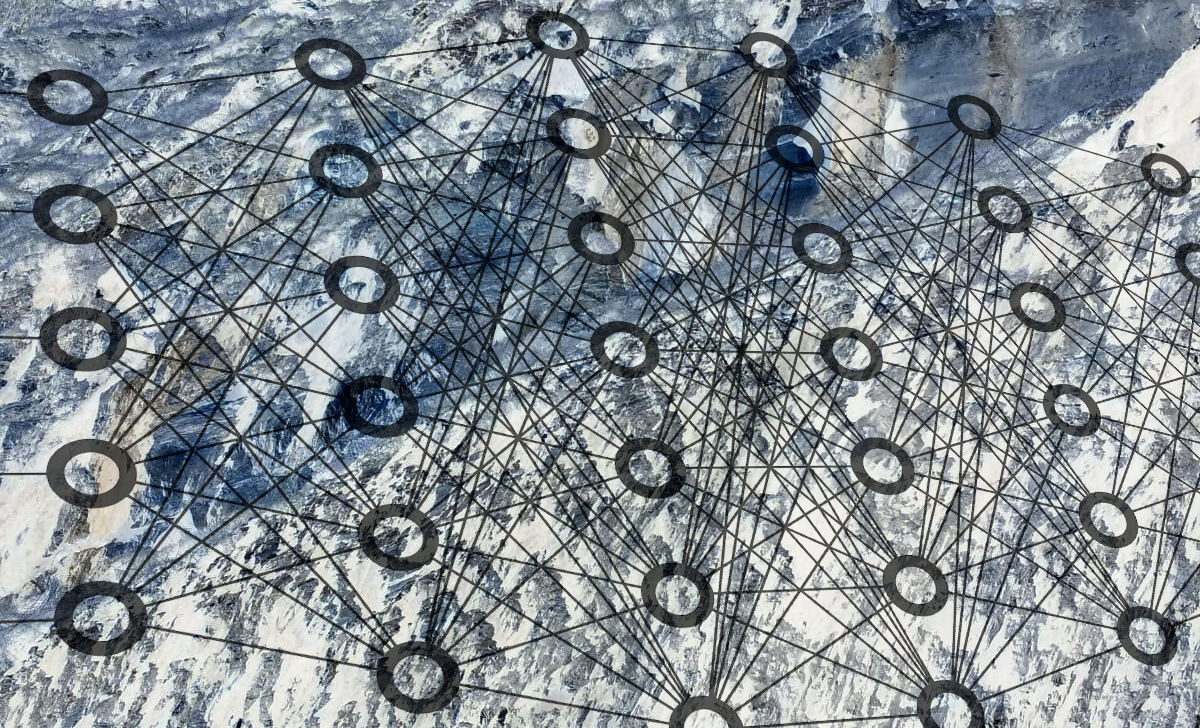
\includegraphics[height=\paperheight,width=\paperwidth]{frames/auxiliar/title_img/prueba.png}};}

\begin{frame}[plain]
\vspace{1cm}
\titlepage

\vspace{-0.2cm}

\includegraphics[height=0.2\textheight]{frames/auxiliar/title_img/upv_transparente.png} \hspace*{7.2cm}

\includegraphics[height=0.2\textheight]{frames/auxiliar/title_img/bcam_transparente.png} \hspace*{0.2cm}
\end{frame} 

}
%%%%%%%%%%%%%%%%%%%%%%%%%%%%%%%%%%
%%%%%%%%%%%%%%%%%%%%%%%%%%%%%%%%%%
%%%%%%%%%%%%%%%%%%%%%%%%%%%%%%%%%%
\begin{section}{Geophysical Problems} 
% Motivation frame
\begin{frame}
    \frametitle{Electromagnetic (EM) Applications}
    \begin{figure}
        \centering
        \begin{subfigure}[b]{0.4\textwidth}
            \centering
            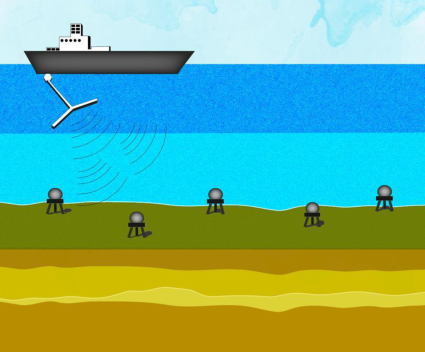
\includegraphics[width=\textwidth]{Diapos/Intro/Figures/csem}
            \caption{CSEM (artificial source)}
        \end{subfigure}
        \hfill
        \begin{subfigure}[b]{0.4\textwidth}
            \centering
            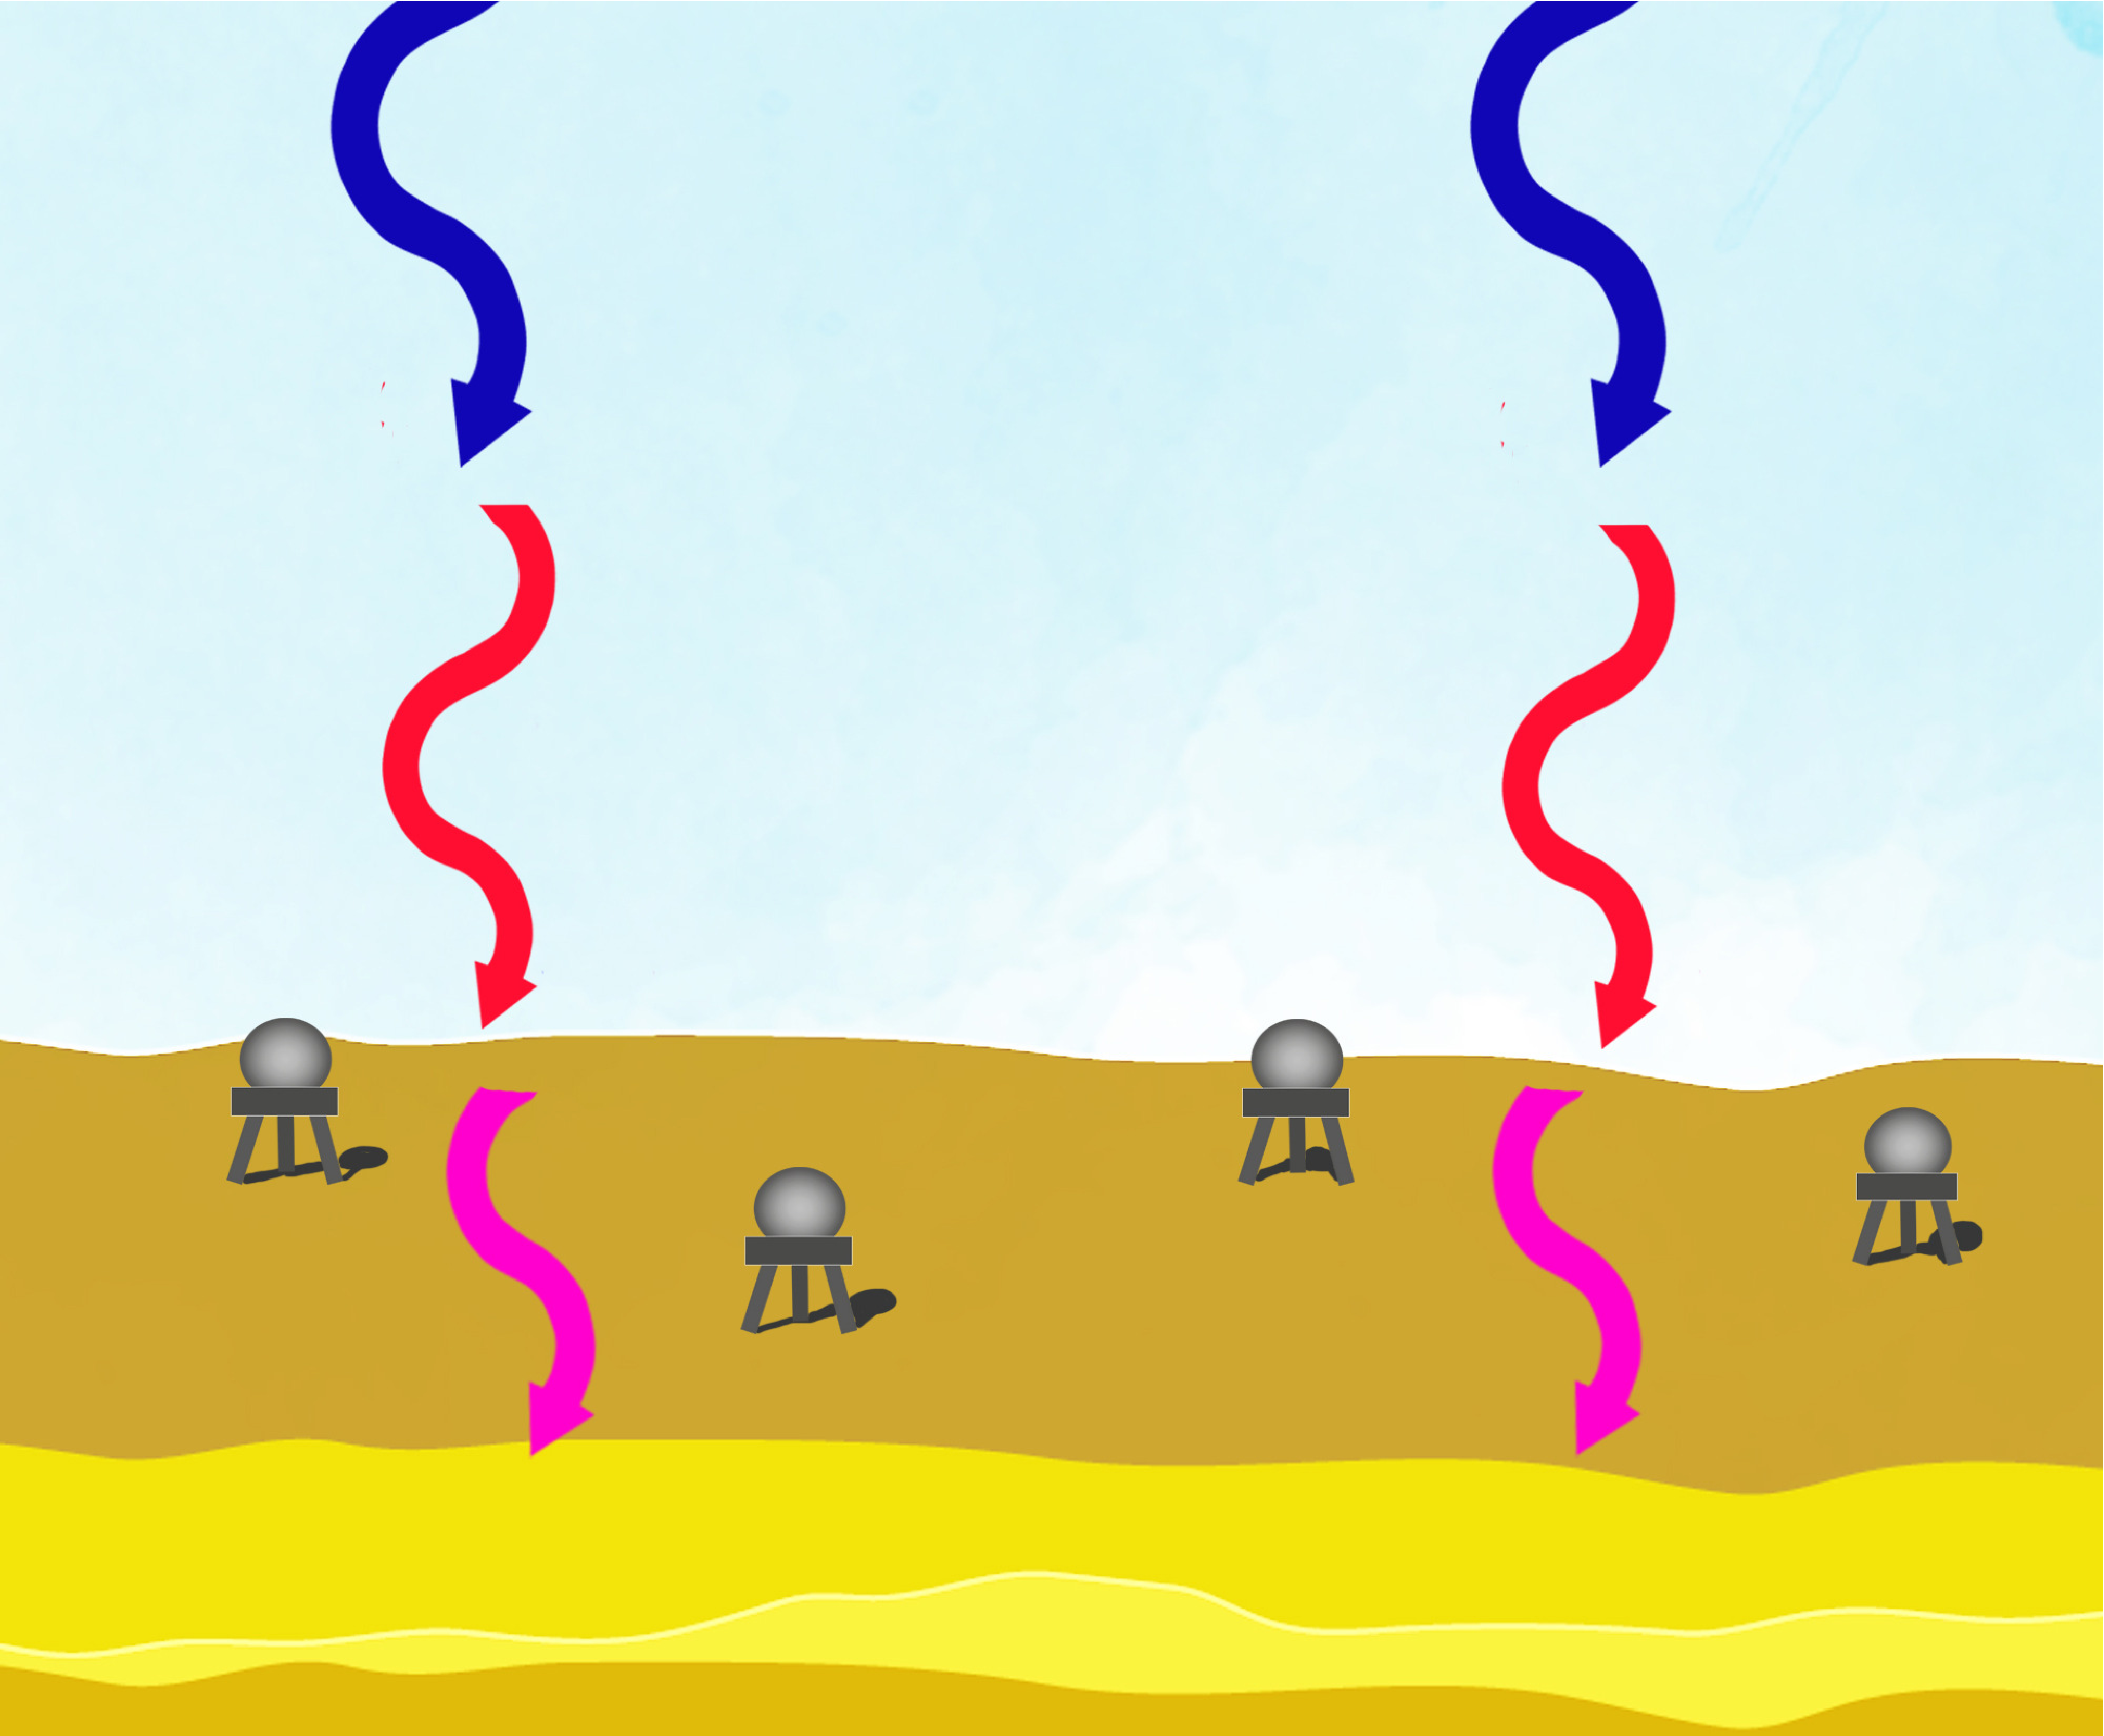
\includegraphics[width=\textwidth]{Diapos/Intro/Figures/magneto}
            \caption{MT (natural source)}
        \end{subfigure}
    \end{figure}
    \vfill
    \begin{block}{Objective}
        \centering
        \textbf{\textcolor{red}{Objective}}: To obtain the \textbf{conductivity/resistivity} distribution of the Earth's subsurface.
    \end{block}
\note[Deep Learning inversion has shown promising results in solving CSEM and MT problems, but it requires large databases for training.]

\end{frame}
\begin{frame}{Overview of Forward and Inverse Problems}
\begin{columns}
\begin{column}{0.35\textwidth}
\begin{tikzpicture}[x=0.8cm, y=0.8cm]
%Material   Block A
\draw[very thin,rounded corners=2pt, fill=orange!30!white ] (-1.5,0) rectangle (1.5,1);
\node[color=black] at (0,0.5) {\footnotesize \textcolor{black}{\textbf{\begin{tabular}{c} Physical \\ properties $(\boldsymbol{m})$ \end{tabular}}}};
%Measurments Block C
\draw[very thin,rounded corners=2pt, fill=orange!30!white ] (-1.5,-8) rectangle (1.5,-7);
\node[color=black] at (0,-7.5) {\footnotesize \textcolor{black}{\textbf{\begin{tabular}{c} Measurements \\ $(\boldsymbol{d})$ \end{tabular}}}};
%%PDE -- Block U
%\draw[very thin,rounded corners=2pt, fill=black ] (4.5,0) rectangle (5.5,1);
\draw[very thin, fill=blue!40!white] (0,-3.5) ellipse (0.5 and 0.5);
\node[color=black] at (0,-3.5) {\footnotesize \textcolor{black}{\textbf{\begin{tabular}{c} u \end{tabular}}}};
%
%%Define some nodes for origen-destination
\node (Aup) at (0,1) {};
\node (Adw) at (0,0) {};
\node (Ar) at (1.5,0.5) {};
\node (Al) at (-1.5,0.5) {};
%
\node (Cup) at (0,-7) {};
\node (Cdw) at (0,-8) {};
\node (Cr) at (1.5,-7.5) {};
\node (Cl) at (-1.5,-7.5) {};
%
\node (Uup) at (0,-3) {};
\node (Udw) at (0,-4) {};
%%arrows
\draw [<-,very thick, draw = green!40!black, postaction={decorate,decoration={raise=1ex,text along path,text align=center,text={|\color{green!40!black}\sffamily|Inverse Problem}}}] (Ar) to [bend left=35] (Cr);
%
\draw [<-,very thick, draw = red, postaction={decorate,decoration={raise=1ex,text along path,text align=center,text={|\color{red}\sffamily|Forward Problem}}}] (Cl) to [bend left=35] (Al);
%
\draw [<-,draw = black, very thick,] (Uup) to [bend left=0]  (Adw);
%
\draw [<-,draw = black, very thick, ] (Cup) to [bend left=0]  (Udw);
%
\fill[fill=white] (-1.5,-5.2) rectangle (1.5,-5.8);
\node at (0,-5.5) {\footnotesize Post-processing};
\fill[fill=white] (-1.5,-1.2) rectangle (1.5,-1.8);
\node at (0,-1.5) {\footnotesize Solve PDE};
\end{tikzpicture}
\end{column}
%
\begin{column}{0.55\textwidth}
\vspace{0,15cm}
\begin{block}{Definitions}
\begin{equation*}
  \begin{array}{cll}
    \mathcal{F} &: & \text{Forward Operator} \\
    & & \boldsymbol{m} \mapsto \boldsymbol{d} \\[2mm]
   \mathcal{I} &: & \text{Inverse Operator} \\
    & & \boldsymbol{d} \mapsto \boldsymbol{m} \\[2mm]
    \mathcal{I}_{\phi} &: & \text{Neural Network approximation of } \mathcal{I}
  \end{array}
\end{equation*}
\end{block}

\end{column}
\end{columns}
\end{frame}

% The arrows indicating the "Inverse Problem" and "Forward Problem" are reversed, as the inverse problem typically goes from data to model, and the forward problem from model to data.
\begin{frame}
    \frametitle{Generation of Massive Databases}    
\vspace{-2mm}

\begin{block}{Objective}
	\centering
	To build a branch of the \textbf{Inverse Operator} (not just to evaluate it).
\end{block}

\begin{block}{Loss Function and Training}
Find $\mathcal{I}_{\phi^*}$ such that
\[
\phi^* = \argmin_{\phi \in \boldsymbol{\Phi}} \sum \left\| (\textcolor{red}{\mathcal{F}} \circ \mathcal{I}_{\phi})(\boldsymbol{d}_i) - \boldsymbol{d}_i \right\|^2
\]
where evaluating $\textcolor{red}{\mathcal{F}}$ is \textcolor{red}{expensive}!
\end{block}
    
\begin{block}{Difficulties}
    \begin{enumerate}
        \item We need a Forward Solver \textcolor{red}{$\mathcal{F}$} for \textcolor{red}{any parameterization} (model).
        \item \textcolor{red}{A huge number} of evaluations is needed \textcolor{red}{to train} the DNN.
    \end{enumerate}
\end{block}

\begin{block}{Solution}
    \begin{enumerate}
        \item  \textcolor{red}{Approximate} the Forward Operator with a  \textcolor{red}{Neural Network}.
    \end{enumerate}
\end{block}

\end{frame}

\begin{frame}{Traditional Numerical Methods in Geophysics}
  \begin{columns}[T,onlytextwidth]
  
    \begin{column}{0.48\textwidth}
      \begin{figure}
        \centering % This ensures the image is centered in the column
        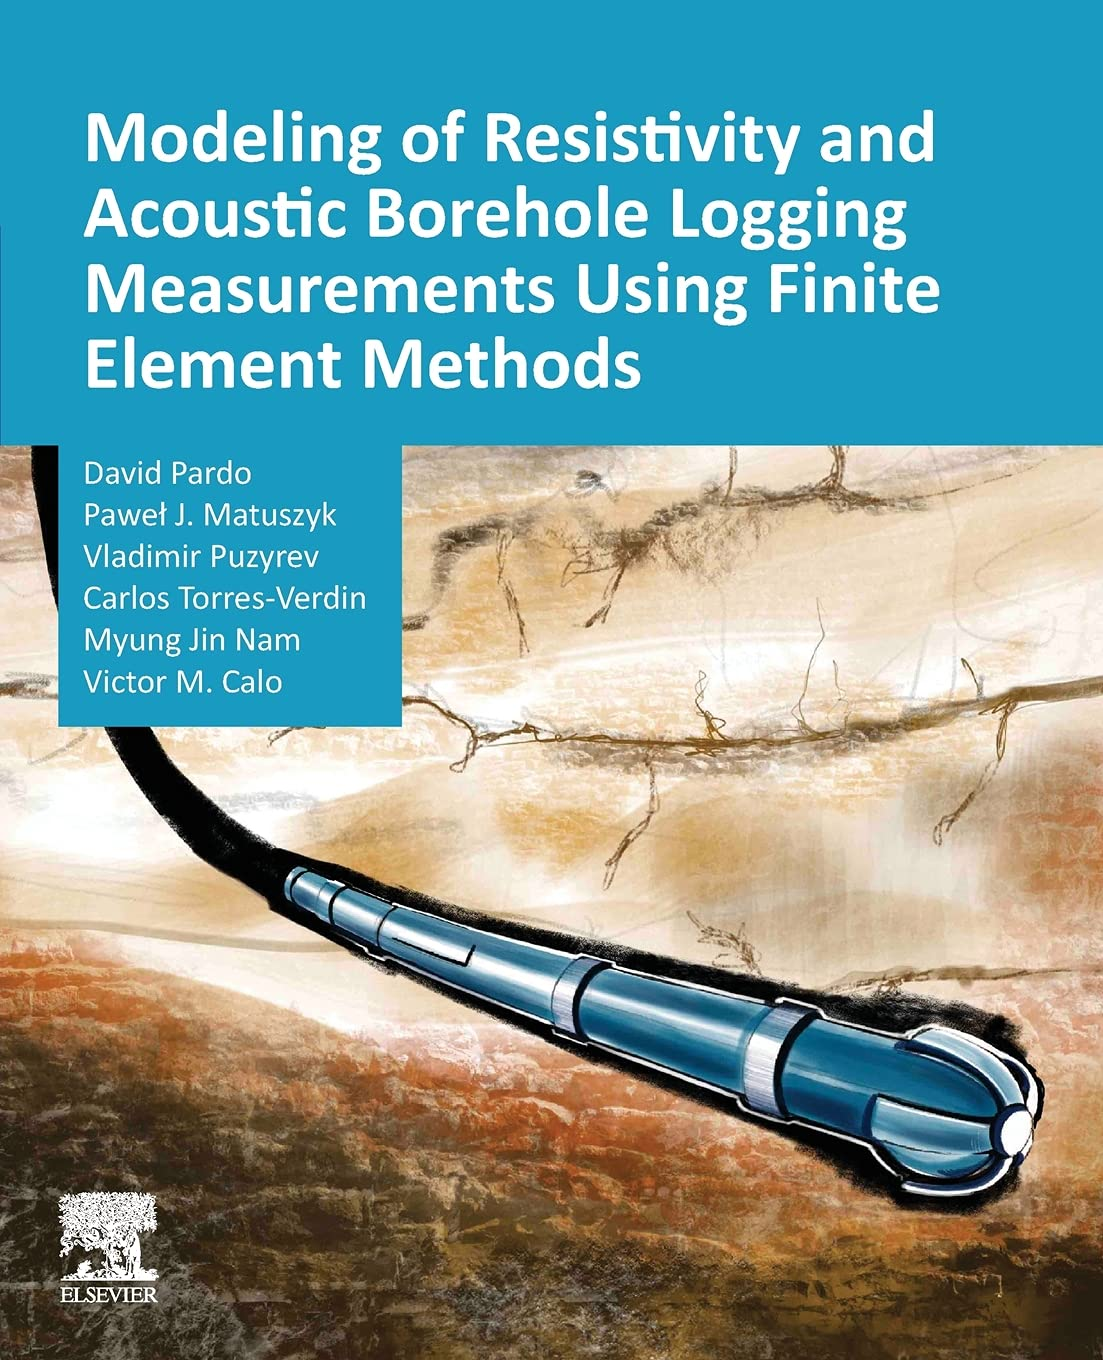
\includegraphics[width=0.8\textwidth]{Diapos/Intro/Figures/PardoBook.jpg} % Using width=\textwidth instead of scale
        \caption{Published in 2021} % Optional caption for the figure
        \label{fig:book} % Label for referencing the figure if needed
      \end{figure}
    \end{column}
    
    \begin{column}{0.48\textwidth}
      \begin{block}{Numerical Methods}
        \begin{itemize}
          \setlength\itemsep{2.4em} % Adjust the space between items
          \item Finite Element method
          \item Finite Difference method
          \item Finite Volumes method
          \item Integral methods
          \item Semi-analytical methods
        \end{itemize}
      \end{block}
    \end{column}
    
  \end{columns}
\end{frame}

\end{section}
%%%%%%%%%%%%%%%%%%%%%%%%%%%%%%%%%%
{
\usebackgroundtemplate{\tikz\node[opacity=0.07,inner sep=0] {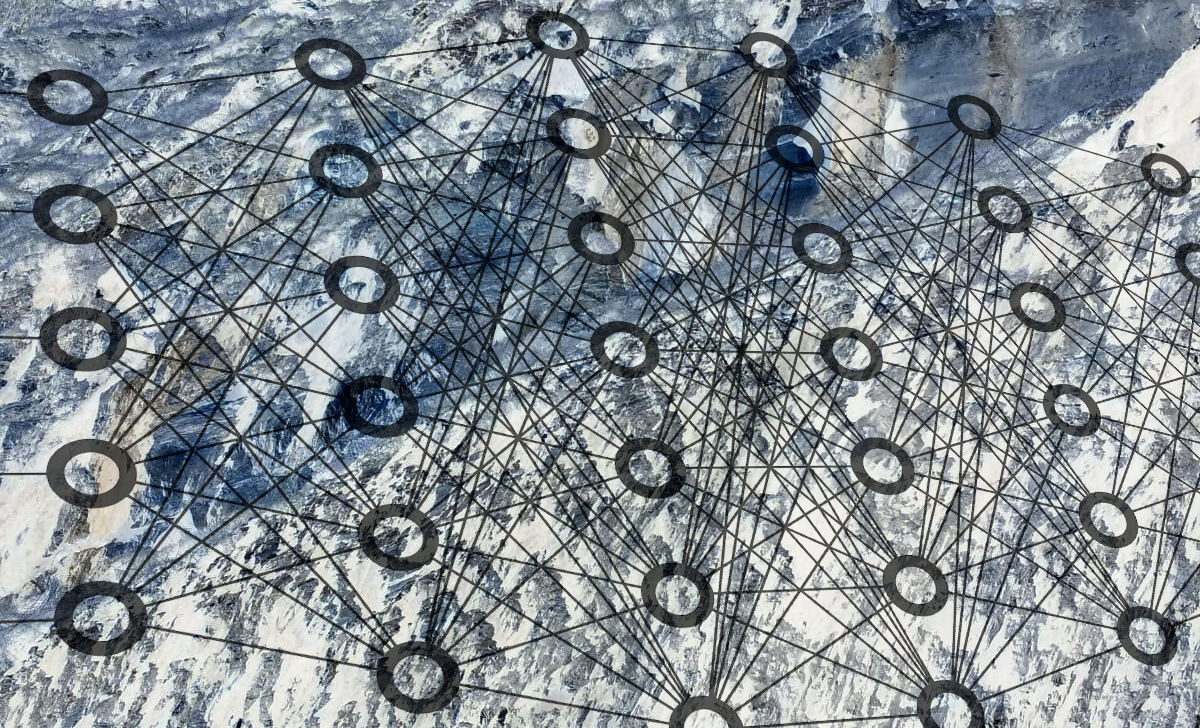
\includegraphics[height=\paperheight,width=\paperwidth]{frames/auxiliar/title_img/prueba.png}};}

\begin{frame}{Outline}
\begin{columns}
\begin{column}{0.05\textwidth}
\end{column}
\begin{column}{0.95\textwidth}

\mybullet{1}{Why Use Deep Learning?}

\vspace{0.4cm}

\mybullet{2}{Deep Learning for Solving Inverse and Forward Problems}

\vspace{0.4cm}

\mybullet{3}{Database Generation using rIGA}
%	\vspace{-0.2cm}
%	\begin{itemize}\setlength{\itemindent}{1cm}
%	\item Existing methods
%	\item Limitation for geophysical problems
%	\item Challenges: Integration, and Minimization
%	\end{itemize}

\vspace{0.4cm}

\mybullet{4}{Solving Forward Problems (PDEs) with Neural Networks}
%	\vspace{-0.2cm}
%	\begin{itemize}\setlength{\itemindent}{1cm}
%	\item Deep Finite Element Method
%	\item $r-$adaptivity with Deep Learning
%	\item Building the Riesz Operator with Deep Methods
%	\item Deep Fourier Method
%\end{itemize}


\vspace{0.4cm}

\mybullet{5}{Achievements}

\vspace{0.4cm}

\mybullet{6}{Conclusions and Future Work}
\end{column}
\end{columns}

\end{frame} 
}
%%%%%%%%%%%%%%%%%%%%%%%%%%%%%%%%%%
\begin{section}{Goal-Oriented $hp$-adaptivity for non-parametric PDEs}
{
\usebackgroundtemplate{\tikz\node[opacity=0.1,inner sep=0] {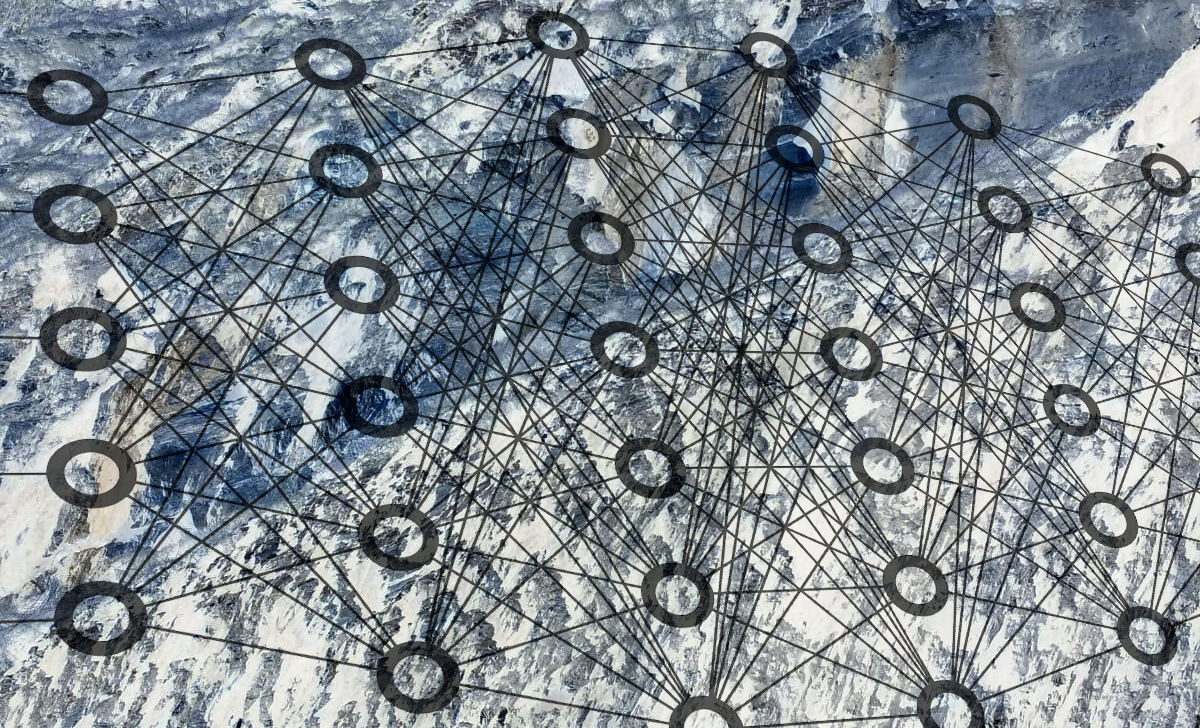
\includegraphics[height=\paperheight,width=\paperwidth]{frames/auxiliar/title_img/prueba.png}};}
%%%%%%%%
\begin{frame}[plain]
\begin{variableblock}{}{bg=myblue,fg=white}{bg=green,fg=red}
\begin{center}
\textbf{Goal-Oriented $hp$-adaptivity for non-parametric PDEs}
\end{center}
\end{variableblock}
\end{frame}
%%%%%%%%%%%%%%%%%%%%%%%%%%%%%%%%%%%%%%%%%%%%%%%%%%%%%%%%%%%%%%%%%%%
}
\newsavebox{\Advantages}
\sbox{\Advantages}{%
\scalebox{0.9}{% Add your desired scale factor here
    \begin{tikzpicture}
        \node[rounded rectangle, draw, ultra thick, color=green!50!black, align=center](Expo){\( hp \)-adaptive FEM\\achieves exponential\\convergence rates};
        \node[below = of Expo, rounded rectangle, draw, ultra thick, color=green!50!black, align=center](Feat){Precise mesh refinement\\near singularities};
        \node[below = of Feat, rounded rectangle, draw, ultra thick, color=green!50!black, align=center](Cheap){Smaller meshes with\\higher accuracy per\\number of degrees of freedom};
        \node[fit=(Feat)(Expo)(Cheap), rectangle, rounded corners, draw, ultra thick, inner sep=1em](adv){};
        \node[anchor=center, rounded corners, draw, thick, fill=white] at (adv.north){Advantages};
    \end{tikzpicture}
}
}

\newsavebox{\limitations}
\sbox{\limitations}{%
\scalebox{0.9}{% Add your desired scale factor here
    \begin{tikzpicture}
        \node[rounded rectangle, draw, ultra thick, color=red, align=center](Mesh){Solution accuracy\\heavily mesh-dependent,\\requiring precise\\mesh design};
        \node[below= of Mesh, rounded rectangle, draw, ultra thick, color=red, align=center](Accuracy){Increasing accuracy\\leads to prohibitive\\computational costs};
        \node[fit=(Mesh)(Accuracy), rectangle, rounded corners, draw, ultra thick, inner sep=1em](limit){};
        \node[anchor=center, rounded corners, draw, thick, fill=white] at (limit.north){Limitations};
    \end{tikzpicture}
}
}

\begin{frame}
    \frametitle{Why \( hp \)-Adaptivity?}
    \begin{center}
        \begin{tikzpicture}
            \node(advan){\usebox{\Advantages}};
            \node[right=2cm of advan](lim){\usebox{\limitations}}; % Adjust the spacing as needed
        \end{tikzpicture}
    \end{center}
\end{frame}
\begin{frame}
	\frametitle{Main Ingredients}
	\begin{figure}
  	\hspace{-1cm}
	\centering
  	\begin{tikzpicture}
    \node[rounded rectangle, draw, ultra thick, align=center] (hp) {
        $hp$-adaptivity
    };
    \node[below left=of hp, circle, minimum size=3cm, draw, ultra thick, align=center] (Data) {
        Data Structures
    };
    \node[below right=of hp, circle, minimum size=3cm, draw, ultra thick, align=center] (Estim) {
        Automatic\\Adaptive\\Strategy
    };

    \draw[->, ultra thick] (hp) -- (Data);
    \draw[->, ultra thick] (hp) -- (Estim);
\end{tikzpicture}

	\caption{Main ingredients}
	\end{figure}	
\end{frame}
\begin{frame}
	\frametitle{Multi-Level Mesh Data Structure 1D}
	\begin{figure}
	\centering
		\begin{tikzpicture}[x=4cm,y=2cm,decoration={markings,% switch on markings mark=% actually add a mark
     	mark=at position 0 with{\draw (0pt,-2pt) -- (0pt,2pt);},
     	mark=at position 1 with{\draw (0pt,-2pt) -- (0pt,2pt);},
	}
	]
	\node(origin1) at (0,1) {};
	\node(origin2) at (1,1) {};
	\node(origin3) at (2,1) {};

	\node(father1) at (0,0) {};
	\node(father2) at (0.25,0) {};
	\node(father3) at (0.5,0) {};
\node(father4) at (0.75,0) {};
\node(father5) at (1,0) {};
\node(father6) at (1.25,0) {};
\node(father7) at (1.5,0) {};
\node(father8) at (1.75,0) {};
\node(father9) at (2,0) {};
\node(father10) at (2.25,0) {};
\node(father11) at (2.5,0) {};
\node(father12) at (2.75,0) {};
\node(father13) at (3,0) {};

\node(son1) at (0,-1) {};
\node(son1a) at (0.125,-1) {};
\node(son1b) at (0.25,-1) {};
\node(son1c) at (0.375,-1) {};
\node(son2)  at (0.5,-1) {};
\node(son3)  at (0.75,-1) {};
\node(son4)  at (1,-1) {};
\node(son10)  at (2,-1) {};
\node(son11) at (2.25,-1) {};
\node(son12) at (2.5,-1) {};
\node(son13) at (2.75,-1) {};
\node(son14) at (3,-1) {};

\node(grandson1) at (0,-2) {};
\node(grandson2)  at (0.25,-2) {};
\node(grandson3)  at (0.5,-2) {};
\node(grandson4)  at (0.625,-2) {};
\node(grandson5)  at (0.75,-2) {};
\node(grandson6)  at (0.875,-2) {};
\node(grandson7)  at (1,-2) {};
\node(grandson8)  at (1.25,-2) {};

\node(ggson1) at (0,-3) {};
\node(ggson2)  at (0.25,-3) {};
\node(ggson3)  at (0.5,-3) {};
\node(ggson4)  at (0.625,-3) {};
\node(ggson5)  at (0.75,-3) {};
\node(ggson6)  at (0.875,-3) {};
\node(ggson7)  at (1,-3) {};
\node(ggson8)  at (1.25,-3) {};


\node(basis0_0) at ($(father1)+(0,0.5)$){};
\node(basis0_1) at ($(father5)+(0,0.5)$){};
\node(basis0_2) at ($(father9)+(0,0.5)$){};
\node(basis0_3) at ($(father13)+(0,0.5)$){};
\node(basis1_1) at ($(son2)+(0,0.5)$){};
\node(basis1_2) at ($(son11)+(0,0.5)$){};
\node(basis1_3) at ($(son12)+(0,0.5)$){};
\node(basis1_4) at ($(son13)+(0,0.5)$){};
\node(basis2_1) at ($(grandson5)+(0,0.5)$){};
\node(basis2_2) at ($(grandson8)+(0,0.5)$){};
\node(basis2_3) at ($(grandson4)+(0,0.25)$){};
\node(basis2_4) at ($(grandson6)+(0,0.25)$){};
\node(basis3_1) at ($(ggson5)+(0,0.5)$){};
\node(basis3_2) at ($(ggson8)+(0,0.5)$){};
\node(basis3_3) at ($(ggson4)+(0,0.5)$){};
\node(basis3_4) at ($(ggson6)+(0,0.5)$){};


%%%%%% HORIZONTAL LINES
% level 1
\draw [postaction={decorate}] (father1.center) -- (father5.center) node[pos=0.5](elemfather1){};
\draw [postaction={decorate}] (father5.center) -- (father9.center) node[pos=0.5](elemfather2){};
\draw [postaction={decorate}] (father9.center) -- (father13.center) node[pos=0.5](elemfather3){};

% level 2

\draw [postaction={decorate,red}] (son1.center) -- (son2.center) node[pos=0.5](elemson1){};
\draw [postaction={decorate}] (son2.center) -- (son4.center) node[pos=0.5](elemson2){};

\draw [postaction={decorate,red}] (son10.center) -- (son12.center) node[pos=0.5](elemson31){};
\draw [postaction={decorate}] (son12.center) -- (son14.center) node[pos=0.5](elemson4){};

% level 2
\draw [postaction={decorate}] (grandson3.center) -- (grandson5.center) node[pos=0.5](elemgrandson1){};
\draw [postaction={decorate}] (grandson5.center) -- (grandson7.center) node[pos=0.5](elemgrandson2){};

% k3
%\draw [postaction={decorate}] (ggson3.center) -- (ggson5.center) node[pos=0.5](elemggson1){};
%\draw [postaction={decorate}] (ggson5.center) -- (ggson7.center) node[pos=0.5](elemggson2){};

%%%%%%%%% BOTTOM LINE %%%%%%%%%

\node(gggson1) at (0,-2.5) {};
\node(gggson2)  at (0.125,-2.5) {};
\node(gggson3)  at (0.25,-2.5) {};
\node(gggson4)  at (0.375,-2.5) {};
\node(gggson5)  at (0.5,-2.5) {};
\node(gggson6)  at (0.625,-2.5) {};
\node(gggson7)  at (0.75,-2.5) {};
\node(gggson8a)  at (0.8125,-2.5) {};
\node(gggson8)  at (0.875,-2.5) {};
\node(gggson8b)  at (0.9325,-2.5) {};
\node(gggson9)  at (1,-2.5) {};
\node(gggson10)  at (1.125,-2.5) {};
\node(gggson11)  at (1.25,-2.5) {};
\node(gggson12)  at (1.375,-2.5) {};
\node(gggson13)  at (1.5,-2.5) {};
\node(gggson14)  at (1.625,-2.5) {};
\node(gggson15)  at (1.75,-2.5) {};
\node(gggson16)  at (1.875,-2.5) {};
\node(gggson17)  at (2,-2.5) {};
\node(gggson18)  at (2.125,-2.5) {};
\node(gggson19)  at (2.25,-2.5) {};
\node(gggson20)  at (2.375,-2.5) {};
\node(gggson21)  at (2.5,-2.5) {};
\node(gggson22)  at (2.625,-2.5) {};
\node(gggson23)  at (2.75,-2.5) {};
\node(gggson24)  at (2.875,-2.5) {};
\node(gggson25)  at (3,-2.5) {};

\draw [|-] (gggson1.center) -- (gggson5.center) node[pos=0.5](){};
\draw [|-] (gggson5.center) -- (gggson7.center) node[pos=0.5](){};
\draw [|-] (gggson7.center) -- (gggson9.center) node[pos=0.5](){};
\draw [|-] (gggson9.center) -- (gggson17.center) node[pos=0.5](){};
\draw [|-] (gggson17.center) -- (gggson21.center) node[pos=0.5](){};
\draw [|-|] (gggson21.center) -- (gggson25.center) node[pos=0.5](){};


%%%%%%%%% VERTICAL LINES %%%%%%%%%

% From level 0
\draw[dotted] (father1.center) -- (gggson1.center);
\draw[dotted] (father5.center) -- (gggson9.center);
\draw[dotted] (father9.center) -- (gggson17.center);
\draw[dotted] (father13.center) -- (gggson25.center);

%\draw[loosely dotted,very thin] (father6.center) -- (gggson11.center);
%\draw[loosely dotted,very thin] (father7.center) -- (gggson13.center);
%\draw[loosely dotted,very thin] (father8.center) -- (gggson15.center);
%\draw[loosely dotted,very thin] (father11.center) -- (gggson21.center);

% From level 1
\draw[loosely dotted] (son2.center) -- (gggson5.center);
%\draw[loosely dotted] (son4.center) -- (gggson9.center);

%\draw[loosely dotted, very thin] (son1a.center) -- (gggson2.center);
%\draw[loosely dotted, very thin] (son1b.center) -- (gggson3.center);
%\draw[loosely dotted, very thin] (son1c.center) -- (gggson4.center);
%\draw[loosely dotted, very thin] (son11.center) -- (gggson19.center);
\draw[loosely dotted, very thin] (son12.center) -- (gggson21.center);
%\draw[loosely dotted, very thin] (son13.center) -- (gggson23.center);


% From level 2
\draw[loosely dotted] (grandson5.center) -- (gggson7.center);

%\draw[loosely dotted, very thin] (ggson4.center) -- (gggson6.center);
%\draw[loosely dotted, very thin] (ggson6.center) -- (gggson6.center);
%\draw[loosely dotted, very thin] (ggson6.center) -- (gggson8.center);

%\node at (gggson1)  {\Cross};
%\node at (gggson2)  {\Cross};
%\node at (gggson3)  {\Cross};
%\node at (gggson4)  {\Cross};
%\node at (gggson5)  {\Cross};
%\node at (gggson6)  {\Cross};
%\node at (gggson7)  {\Cross};
%\node at (gggson8a)  {\Cross};
%\node at (gggson8)  {\Cross};
%\node at (gggson8b)  {\Cross};
%\node at (gggson9)  {\Cross};
%\node at (gggson11)  {\Cross};
%\node at (gggson13)  {\Cross};
%\node at (gggson15)  {\Cross};
%\node at (gggson17)  {\Cross};
%%\node at (gggson19)  {\Cross};
%\node at (gggson21)  {\Cross};
%%\node at (gggson23)  {\Cross};
%\node at (gggson25)  {\Cross};

%%%%%%%%% BASIS FUNCTIONS %%%%%%%%%
%%%%%% level 0

% linear basis function

\draw[color=black, thick] (basis0_0.center) -- (father5.center);
\draw[color=black, thick] (father1.center) -- (basis0_1.center) -- (father9.center);
\draw[color=black, thick] (father5.center) -- (basis0_2.center) -- (father13.center);
\draw[color=black, thick] (basis0_3.center) -- (father9.center);

% degree 2 basis function
\draw[color=black, thick]    (father5.center) .. controls ($(elemfather2)+(-0.05,+0.15)$) and ($(elemfather2)+(0.05,0.15)$) ..  (father9.center) ;
%\draw[color=black, thick]    (father9.center) .. controls ($(elemfather3)+(-0.05,+0.15)$) and ($(elemfather3)+(0.05,0.15)$) ..  (father13.center) ;

% degree 3 basis function
\draw[color=blue, ultra thick]   (father5.center) .. controls ($(elemfather2)+(-0.01,-0.25)$) and ($(elemfather2)+(0.00,0.25)$) ..  (father9.center);

%%%%% level 1
% linear basis function
\draw[color=black, thick] (son1.center) -- (basis1_1.center) -- (son4.center);
\draw[color=blue, ultra thick] (son10.center) -- (basis1_3.center) -- (son14.center);
%\draw[color=red, thick] (son10.center) -- (basis1_2.center) -- (son12.center);
%\draw[color=red, thick] (son12.center) -- (basis1_4.center) -- (son14.center);

% degree 2 basis function
\draw[color=black, thick]    (son1.center) .. controls ($(elemson1)+(-0.05,+0.15)$) and ($(elemson1)+(0.05,0.15)$) ..  (son2.center);

% degree 3 basis function
\draw[color=blue, ultra thick]   (son1.center) .. controls ($(elemson1)+(-0.0,-0.25)$) and ($(elemson1)+(0.0,0.25)$) ..  (son2.center);


%%%%% level 2

% linear basis function
\draw[color=black, thick] (grandson3.center) -- (basis2_1.center) -- (grandson7.center);
%\draw[color=red, thick]    (grandson3.center) -- (basis2_3.center) -- (grandson5.center);
%\draw[color=red, thick]    (grandson5.center) -- (basis2_4.center) -- (grandson7.center);

% degree 2 basis function
\draw[color=blue, ultra thick]    (grandson3.center) .. controls ($(elemgrandson1)+(-0.05,+0.15)$) and ($(elemgrandson1)+(0.05,0.15)$) ..  (grandson5.center);
\draw[color=black, thick]    (grandson5.center) .. controls ($(elemgrandson2)+(-0.05,+0.15)$) and ($(elemgrandson2)+(0.05,0.15)$) ..  (grandson7.center);

% degree 3 basis function
\draw[color=blue, ultra thick]   (grandson5.center) .. controls ($(elemgrandson2)+(-0.0,-0.25)$) and ($(elemgrandson2)+(0.0,0.25)$) ..  (grandson7.center);


%%%%% k3

% linear basis function
%\draw[color=red, thick]    (ggson3.center) -- (basis3_3.center) -- (ggson5.center);
%\draw[color=red, thick]    (ggson5.center) -- (basis3_4.center) -- (ggson7.center);

%%%%%%%%% CIRCLES %%%%%%%%%

%%%%%% level 0

\node[circle,draw, fill=black, inner sep=0pt,minimum size=5pt] at ($(father1)+(0,0)$){};
%\node[circle,draw, fill=white, inner sep=0pt,minimum size=5pt] at ($(father1a)+(0,0)$){};
%\node[circle,draw, fill=white, inner sep=0pt,minimum size=5pt] at ($(father1b)+(0,0)$){};
\node[circle,draw, fill=black, inner sep=0pt,minimum size=5pt] at ($(father5)+(0,0)$){};
%\node[circle,draw, fill=black, inner sep=0pt,minimum size=5pt] at ($(father6)+(0,0)$){};
%\node[circle,draw, fill=black, inner sep=0pt,minimum size=5pt] at ($(father7)+(0,0)$){};
%\node[circle,draw, fill=black, inner sep=0pt,minimum size=5pt] at ($(father8)+(0,0)$){};
\node[circle,draw, fill=black, inner sep=0pt,minimum size=5pt] at ($(father9)+(0,0)$){};
%\node[circle,draw, fill=black, inner sep=0pt,minimum size=5pt] at ($(father11)+(0,0)$){};
\node[circle,draw, fill=black, inner sep=0pt,minimum size=5pt] at ($(father13)+(0,0)$){};

%%%%%% level 1

\node[circle,draw, fill=white, inner sep=0pt,minimum size=5pt] at ($(son1)+(0,0)$){};

%\node[circle,draw, fill=black, inner sep=0pt,minimum size=5pt] at ($(son1a)+(0,0)$){};
%\node[circle,draw, fill=black, inner sep=0pt,minimum size=5pt] at ($(son1b)+(0,0)$){};
%\node[circle,draw, fill=black, inner sep=0pt,minimum size=5pt] at ($(son1c)+(0,0)$){};
\node[circle,draw, fill=black, inner sep=0pt,minimum size=5pt] at ($(son2)+(0,0)$){};
\node[circle,draw, fill=white, inner sep=0pt,minimum size=5pt] at ($(son4)+(0,0)$){};
\node[circle,draw, fill=white, inner sep=0pt,minimum size=5pt] at ($(son10)+(0,0)$){};
%\node[circle,draw, fill=black, inner sep=0pt,minimum size=5pt] at ($(son11)+(0,0)$){};
\node[circle,draw, fill=black, inner sep=0pt,minimum size=5pt] at ($(son12)+(0,0)$){};
%\node[circle,draw, fill=black, inner sep=0pt,minimum size=5pt] at ($(son13)+(0,0)$){};
\node[circle,draw, fill=white, inner sep=0pt,minimum size=5pt] at ($(son14)+(0,0)$){};

%%%%%% level 2
\node[circle,draw, fill=white, inner sep=0pt,minimum size=5pt] at ($(grandson3)+(0,0)$){};
%\node[circle,draw, fill=black, inner sep=0pt,minimum size=5pt] at ($(grandson4)+(0,0)$){};
\node[circle,draw, fill=black, inner sep=0pt,minimum size=5pt] at ($(grandson5)+(0,0)$){};
%\node[circle,draw, fill=black, inner sep=0pt,minimum size=5pt] at ($(grandson6)+(0,0)$){};
\node[circle,draw, fill=white, inner sep=0pt,minimum size=5pt] at ($(grandson7)+(0,0)$){};

%%%%%% level 2
%\node[circle,draw, fill=white, inner sep=0pt,minimum size=5pt] at ($(ggson3)+(0,0)$){};
%\node[circle,draw, fill=black, inner sep=0pt,minimum size=5pt] at ($(ggson4)+(0,0)$){};
%\node[circle,draw, fill=white, inner sep=0pt,minimum size=5pt] at ($(ggson5)+(0,0)$){};
%\node[circle,draw, fill=black, inner sep=0pt,minimum size=5pt] at ($(ggson6)+(0,0)$){};
%\node[circle,draw, fill=white, inner sep=0pt,minimum size=5pt] at ($(ggson7)+(0,0)$){};

%%%%%%%%%%% LEGEND

%\draw[blue, very thick] at (origin) rectangle (3,2);
%\node[rectangle,draw] at (origin1) {};

\node[circle,draw, fill=white, inner sep=0pt,minimum size=5pt] at (origin1){};
\node at ($(origin1) +(0.35,0.01)$)  {Dirichlet nodes};

\node[circle,draw, fill=black, inner sep=0pt,minimum size=5pt] at (origin2){};
\node at ($(origin2) +(0.3,0.01)$)  {Active nodes};

\node[rectangle, inner sep=0pt, minimum height=1pt, minimum width=6pt, draw=blue, fill=blue] at (origin3)  {};
%\node at (origin3)  {\Cross};
\node at ($(origin3) +(0.4,0)$)  {Basis functions};

%%%%%%%%%%%  TEXT

%%%% left  %%%%

%\node[anchor=west] at ($(father1)-(0.9,0)$) {level 0 (base)};
%\node[anchor=west] at ($(son1)-(0.75,0)$) {level 1};
%\node[anchor=west] at ($(grandson1)-(0.75,0)$) {level 2};
%\node[anchor=west] at ($(ggson1)-(0.75,0)$) {level 3};
%\node[anchor=west] at ($(gggson1)-(0.9,0)$) {Overlapped mesh};

%%%% bottom  %%%%

\node at ($(gggson3) +(0,-0.2)$)  {$p=3$};
\node at ($(gggson6) +(0,-0.2)$)  {$p=2$};
\node at ($(gggson8) +(0,-0.2)$)  {$p=3$};
\node at ($(gggson13) +(0,-0.2)$)  {$p=3$};
\node at ($(gggson19) +(0,-0.2)$)  {$p=1$};
\node at ($(gggson23) +(0,-0.2)$)  {$p=1$};



\end{tikzpicture}
	\end{figure}
\end{frame}
\begin{frame}
	\frametitle{Multi-Level Mesh Data Structure 2D}
	\begin{figure}
	\begin{center}
	%\tikzset{/tikz/external/export next=false}
	\begin{tikzpicture}[x=3cm,y=3cm]
	\begin{scope}[%every node/.append style={yslant=0.5,xslant=-1.3},
        yslant=0.5,xslant=-1.3
        ]
	\draw[fill= gray!60!white, line width=1pt] (0,0) rectangle (1.5,1.5);
	\path[fill=white!80!gray, draw] (0.5,0.5) rectangle (1,1);
	\draw[step=1/2, line width=1pt] (0,0) grid (1.5,1.5);

	\foreach \x in {0,0.5,1, 1.5}{
		\foreach \y in {0,0.5,1,1.5}{
			\node[circle, draw, fill=black, inner sep=2pt] at (\x,\y){};
		}
	}
	\node at (0.5,0.5) (root1){};
	\node at (0.5,1) (root2){};
	\node at (1,0.5) (root3){};
	\node at (1,1) (root4){};
	\end{scope}

	\begin{scope}[
	yshift=0.9cm,
	%every node/.append style={yslant=0.5,xslant=-1.3},
        yslant=0.5,xslant=-1.3
        ]
	\node at (0.5,0.5) (son1){};
	\node at (0.5,1) (son2){};
	\node at (1,0.5) (son3){};
	\node at (1,1) (son4){};

	\node at (0.75,0.5) (son5){};
	\node at (0.75,1) (son6){};
	\node at (0.5,0.75) (son7){};
	\node at (1,0.75) (son8){};

	\foreach \i in {1,2,...,4}{
		\draw[dashed] (son\i) -- (root\i);
	}
	
	\path[fill=gray, opacity=0.6] (0.5,0.5) rectangle (1,1);
	\draw[dotted,  line width=1pt] (0.5,0.5) rectangle (1,1);
	\draw[line width=1pt] (son5) -- (son6);
	\draw[line width=1pt] (son7) -- (son8);

	\foreach \xy in { (son5), (son6), (son7) , (son8)}{
		\node[circle, draw, fill=white, inner sep=2pt] at \xy{};
	}
	\node[circle, draw, fill=black, inner sep=2pt] at (0.75,0.75){};

	\path (son3) to node[pos=0.1](pinEdge){} (son4);

	\node[above right =0.2 of pinEdge, anchor=west, inner sep=1pt](legend1){Dirichlet edge};
	\node[above right =0.2 of son8, anchor=south, inner sep=1pt](legend2){Dirichlet node};

	\draw[color=black, thin, shorten <=-3pt,<-] (pinEdge) -- (legend1.south west);
	\draw[color=black, thin, shorten <=-2pt,<-] (son8) -- (legend2.south);
	\end{scope}
	\end{tikzpicture}
	%\missingfigure[figwidth=6cm]{Testing a long text string}
	\end{center}
	\caption{\alert{Multi-level} 2D mesh without constraints on hanging nodes using Dirichlet nodes. The bubble basis functions are at the \alert{lowest level} of each family \label{fig:Multilevel}}
	\end{figure}
	\vfill
	\begin{thebibliography}{10}
	\beamertemplatearticlebibitems
	\scriptsize
	\bibitem{ZanderBog:2015}
	N. Zander, T. Bog, S. Kollmannsberger, D. Schillinger, and E. Rank
	\newblock Multi-level $hp$-adaptivity: high-order mesh adaptivity without the
  	difficulties of constraining hanging nodes
	\newblock \emph{Computational Mechanics}, 55\penalty0 (3):\penalty0 499--517,
  	Mar 2015
	\end{thebibliography}
\end{frame} 
\begin{frame}
    \frametitle{A Painless Automatic Adaptive Strategy}
    
    \begin{figure}
        \centering
        \resizebox{0.55\textwidth}{!}{% Resize to the width of the text block
	\begin{tikzpicture}
		\node[rounded rectangle, draw, very thick](Init) {Initial coarse mesh};
		\node[below right=1/2 of Init,rounded rectangle, draw, very thick,color=blue,align=center](ref) {Arbitrary \\(user-defined/global)\\ refinements};
		\node[below= of ref, rounded rectangle, draw, very thick,color=green!50!black, align=center](unrefProcess) {Quasi-optimal\\$hp$-unrefinements};
		\node[below right=1/2 of unrefProcess,rounded rectangle, draw, very thick](final) {Adapted mesh};

		\draw[->, thick] (Init) -| (ref);
		\draw[->, thick,color=blue] (ref.east) to[out=0,in=0] (unrefProcess.east);
		\draw[->, thick,color=green!50!black] (unrefProcess.west) to[out=180,in=180] node[pos=0.5](PinExitRef){} (ref.west);
		\draw[->, thick] (unrefProcess) |- (final);
	\end{tikzpicture}
}
    \end{figure}

    \begin{thebibliography}{10}
        \beamertemplatearticlebibitems
        \scriptsize
        \bibitem{darrigrand2020painless}
        V. Darrigrand, D. Pardo, T. Chaumont-Frelet, I. G{\'o}mez-Revuelto, L. E. Garc{\'i}a-Castillo
        \newblock A painless automatic $hp$-adaptive strategy for elliptic problems
        \newblock \emph{Finite Elements in Analysis and Design}, 2020.

        \beamertemplatearticlebibitems
        \scriptsize
        \bibitem{caro2022painless}
        F. V. Caro, V. Darrigrand, J. Alvarez-Aramberri, E. Alberdi, D. Pardo
        \newblock A painless multi-level automatic goal-oriented $hp$-adaptive coarsening strategy for elliptic and non-elliptic problems
        \newblock \emph{Computer Methods in Applied Mechanics and Engineering}, 2022.
    \end{thebibliography}
\end{frame}

\begin{frame}
    \frametitle{Quasi-optimal \( hp \)-unrefinements}
    \vfill
    \begin{center}
        \begin{figure}
            \centering
        		\begin{tikzpicture}
                \node[rounded rectangle, draw, very thick] (Solve) {Solve};
                \node[right = of Solve, rounded rectangle, draw, very thick, align=center] (Estimate) {Estimate};
                \node[right =1.2 of Estimate, rounded rectangle, draw, very thick] (Mark) {Mark};
                \node[right = of Mark, rounded rectangle, draw, very thick, align=center] (Update) {Update \\ the mesh};
                \draw[->, very thick] (Solve) -- (Estimate);
                \draw[->, very thick] (Estimate) -- (Mark);
                \draw[->, very thick] (Mark) -- (Update);
                
                \node[below= 1/2 of Estimate, align=center, rounded corners, rectangle, draw, very thick, dashed] (DetailsEstimate) {
                    $\bullet$ Find the {\color{green!50!black} removable} workers\\
                    $\bullet$ Estimate their contribution
                };
                \node[below= 2 of Mark, align=center, rounded corners, rectangle, draw, very thick, dashed] (DetailsMark) {
                    $\bullet$ Mark the {\color{green!50!black} lazy} workers
                };
                \node[below= 3 of Update, align=center, rounded corners, rectangle, draw, very thick, dashed] (DetailsUpdate) {
                    $\bullet$ Fire them
                };

                \draw[->, very thick, dashed] (Estimate) -- (DetailsEstimate);
                \draw[->, very thick, dashed] (Mark) -- (DetailsMark);
                \draw[->, very thick, dashed] (Update) -- (DetailsUpdate);
            \end{tikzpicture}
            \caption{Quasi-optimal \( hp \)-unrefinement steps}
        \end{figure}
    \end{center}    
\end{frame}

\begin{frame}
	\frametitle{Removable 1D Basis Functions}
	\begin{block}{Definition}
	We define {\color{green!50!black} removable} basis functions as those we can eliminate from the discretization without modifying any other basis 	function while preserving \textbf{complete} polynomial spaces. 
	\end{block}
	\begin{figure}
	 \hspace{-1cm}
	\centering
	 \begin{subfigure}[b]{\subplotwidth}
	\centering
	\begin{tikzpicture}[x=2cm,y=2cm,decoration={markings,
     		mark=at position 0 with{\draw (0pt,-2pt) -- (0pt,2pt);},
     		mark=at position 1 with{\draw (0pt,-2pt) -- (0pt,2pt);},
	}
	]

	\node(father1) at (0,0) {};
	\node(father2) at (1,0) {};
	\node(father3) at (2,0) {};

	\node(son1) at (0,-1) {};
	\node(son2)  at (0.5,-1) {};
	\node(son3)  at (1,-1) {};
	\node(son4)  at (1.5,-1) {};
	\node(son5)  at (2,-1) {};

	\node(basis1) at ($(father2)+(0,0.5)$){};
	\node(basis2) at ($(son2)+(0,0.5)$){};
	\node(basis3) at ($(son4)+(0,0.5)$){};

	\draw [postaction={decorate}] (father1.center) -- (father2.center) node[pos=0.5](elemfather1){};
	\draw [postaction={decorate}] (father2.center) -- (father3.center) node[pos=0.5](elemfather2){};

	\draw[dashed] (father1.center) -- (son1.center);
	\draw[dashed] (father2.center) -- (son3.center);

	\draw [postaction={decorate}] (son1.center) -- (son2.center) node[pos=0.5](elemson1){};
	\draw [postaction={decorate}] (son2.center) -- (son3.center) node[pos=0.5](elemson2){};

	\node[anchor=north] at (elemfather1) {};
	\node[anchor=north] at (elemfather2) {};

	\node[anchor=north] at (elemson1) {};
	\node[anchor=north] at (elemson2) {};
	% linear basis function
	\draw[color=red, thick] (father1.center) -- (basis1.center) -- (father3.center);
	\draw[color=red, thick] (son1.center) -- (basis2.center) -- (son3.center);
	% degree 2 basis function
	\draw[color=red, thick]    (son1.center) .. controls ($(elemson1)+(-0.1,+0.15)$) and ($(elemson1)+(0.1,0.15)$) ..  (son2.center) ;
	\draw[color=blue,ultra thick]    (son2.center) .. controls ($(elemson2)+(-0.1,+0.15)$) and ($(elemson2)+(0.1,0.15)$) ..  (son3.center);
	\draw[color=blue,ultra thick]    (father2.center) .. controls ($(elemfather2)+(-0.1,+0.15)$) and ($(elemfather2)+(0.1,0.15)$) ..  (father3.center) ;
	% degree 3 basis function
	\draw[color=blue,ultra thick]   (son1.center) .. controls ($(elemson1)+(-0.1,-0.15)$) and ($(elemson1)+(0.1,0.15)$) ..  (son2.center);
	\end{tikzpicture}
	\caption{$hp$-case\label{fig:basis1Dhp}}
	\end{subfigure}
	\begin{subfigure}[b]{\subplotwidth}
	\centering
	\begin{tikzpicture}[x=2cm,y=2cm,decoration={markings,% switch on markings mark=% actually add a mark
     		mark=at position 0 with{\draw (0pt,-2pt) -- (0pt,2pt);},
     	mark=at position 1 with{\draw (0pt,-2pt) -- (0pt,2pt);},
	}
	]
	\node(father1) at (0,0) {};
	\node(father2) at (1,0) {};
	\node(father3) at (2,0) {};

	\node(son1) at (0,-1) {};
	\node(son2)  at (0.5,-1) {};
	\node(son3)  at (1,-1) {};	
	\node(son4)  at (1.5,-1) {};
	\node(son5)  at (2,-1) {};

	\node(basis1) at ($(father2)+(0,0.5)$){};
	\node(basis2) at ($(son2)+(0,0.5)$){};
	\node(basis3) at ($(son4)+(0,0.5)$){};

	\draw [postaction={decorate}] (father1.center) -- (father2.center) node[pos=0.5](elemfather1){};
	\draw [postaction={decorate}] (father2.center) -- (father3.center) node[pos=0.5](elemfather2){};

	\draw[dashed] (father1.center) -- (son1.center);
	\draw[dashed] (father2.center) -- (son3.center);

	\draw [postaction={decorate}] (son1.center) -- (son2.center) node[pos=0.5](elemson1){};
	\draw [postaction={decorate}] (son2.center) -- (son3.center) node[pos=0.5](elemson2){};

	\node[anchor=north] at (elemfather1) {};
	\node[anchor=north] at (elemfather2) {};

	\node[anchor=north] at (elemson1) {};
	\node[anchor=north] at (elemson2) {};
	% linear basis function
	\draw[color=red, thick]   (father1.center) -- (basis1.center) -- (father3.center);
	\draw[color=blue, ultra thick]   (son1.center) -- (basis2.center) -- (son3.center) ;
	\end{tikzpicture}
	\caption{$h$-case \label{fig:basis1Dh}}
\end{subfigure}
	\caption{Removable 1D basis functions}
	\end{figure}
\end{frame}

\begin{frame}
    \frametitle{Adaptive Mesh Refinement Algorithm}

    \SetKwRepeat{Do}{do}{end}%
    \begin{algorithm}[H]
      \SetAlgoLined
      \KwIn{A given initial mesh}
      \KwOut{A final \(hp\)-adapted mesh}

     \While{error above tolerance}{
        Perform a global and uniform (\(h\) or \(p\)) refinement\;
        Execute a (quasi)-optimal \(hp\)-coarsening step (Algorithm 2) to the mesh\;
        Update error\;
      }
      \caption{Adaptive process}
      \label{alg:adaptive}
    \end{algorithm}
\end{frame}

\begin{frame}
    \frametitle{\( hp \)-Unrefinement Policy}
    \SetKwRepeat{Do}{do}{end}%
    \begin{algorithm}[H]
      \SetAlgoLined
      \KwIn{A given mesh}
      \KwOut{An \( hp \)-unrefined mesh}

      \Do{}{
        Compute the solution on the current mesh\;
        Compute the element-wise error indicators\;
        Unrefine the mesh by eliminating the \emph{removable} basis functions with low error indicators\;
        When no contributions are below a given tolerance, exit\;
      }
      \caption{\( hp \)-unrefinement policy}
      \label{alg:unrefining}
    \end{algorithm}
\end{frame}
\begin{frame}
  \frametitle{Illustrating the Goal-Oriented $hp$-Adaptive Strategy}
  
  \begin{block}{Wave propagation problem}
     Find \(u\) satisfying:
    \begin{alignat}{2}
      - \Delta u -k^{2}u   & = \mathds{1}_{\Omega_{f}} &  & \quad \text{in } \Omega, \label{eq:helmholtzgoal} \\
      u                    & = 0                       &  & \quad \text{on } \Gamma_{D}, \\
      \nabla u \cdot \vec{n} & = 0                     &  & \quad \text{on } \Gamma_{N}.
    \end{alignat}
  \end{block}

  \begin{multicols}{2}
    \textbf{Domain Definitions:}
    \begin{itemize}
      \item \(\Omega_{f} = \left(0,\frac{1}{4}\right)^{2} \subset \Omega\), 
      \item \(k = \left(8 \cdot 2 \pi, 2 \pi\right)\), 
      \item \(\Omega_{l} = \left(\frac{3}{4},1\right)^{2} \subset \Omega\),
    \end{itemize}

   \begin{figure}
       \centering
	 \begin{tikzpicture}[x=2.01cm,y=2.01cm]
        % Nodes definition
        \node(n1) at (0,0){};
        \node(n2) at (1,0){};
        \node(n3) at (1,1){};
        \node(n4) at (0,1){};
        \node(n5) at (0.25,0.25){};
        \node(n6) at (0.75,0.25){};
        \node(n7) at (0.75,0.75){};
        \node(n8) at (0.25,0.75){};

        % Drawing rectangles
        \draw (n1) rectangle (n5) node[pos=0.5] {\footnotesize\( \Omega_{f} \)};
        \draw (n7) rectangle (n3) node[pos=0.5] {\footnotesize\( \Omega_{l} \)};

        % Boundary lines
        \draw[line width=0.5mm, color=blue] (n5) rectangle (n7);
        \draw[line width=0.5mm, color=blue] (n4.center) -- (n1.center) -- (n2.center) node[pos=0.5,pin={-90: \( \Gamma_{D} \)}]{};
        \draw[line width=0.5mm, color=red] (n4.center)--  (n3.center) -- node[pos=0.5,pin={0: \( \Gamma_{N} \)}]{} (n2.center);

        % Pattern filling
        \draw [draw=black, pattern=north west lines, pattern color=gray!50] (n5) rectangle (n7);

        % Label for Omega
        \node(omega) at (0.5,0.85){\( \Omega \)};
\end{tikzpicture}
	      \caption{Domain \(\Omega = \left(0,1\right)^{2} \setminus \left(\frac{1}{4},\frac{3}{4}\right)^{2} \subset \mathbb{R}^{2}\).}
    \end{figure}

  \end{multicols}

\end{frame}

\begin{frame}
	\frametitle{Illustrating the Goal-Oriented $hp$-Adaptive Strategy}
	\begin{figure}[t!]
   		\goasolutions{Helm2DGOA}{abs}
	\end{figure}
\end{frame}

\begin{frame}
	\frametitle{Illustrating the Goal-Oriented $hp$-Adaptive Strategy}
  	\plothpmeshes[]{Helm2DGOA}
\end{frame}
%\begin{frame}
	\frametitle{Illustrating the Goal-Oriented $hp$-Adaptive Strategy}
	\plothpunrefmago{hpmago}
\end{frame}
\end{section}
%%%%%%%%%%%%%%%%%%%%%%%%%%%%%%%%%%
%%%%%%%%%%%%%%%%%%%%%%%%%%%%%%%%%%
\begin{section}{Goal-Oriented coarsening strategy}
%%%%%%%%
{
\usebackgroundtemplate{\tikz\node[opacity=0.1,inner sep=0] {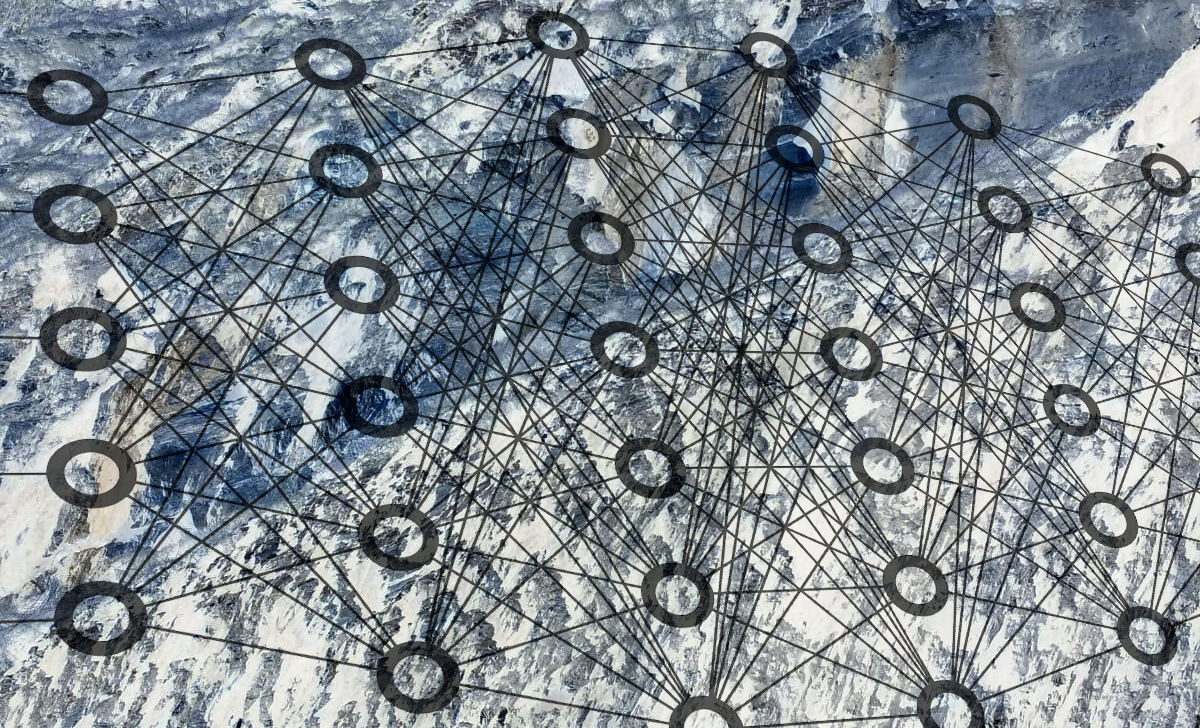
\includegraphics[height=\paperheight,width=\paperwidth]{frames/auxiliar/title_img/prueba.png}};}

\begin{frame}[plain]
\begin{variableblock}{}{bg=myblue,fg=white}{bg=green,fg=red}
\begin{center}
\textbf{Goal-Oriented coarsening strategy}
\end{center}
\end{variableblock}
\end{frame}
}
%%%%%%%%%%%%%%%%%%%%%%%%%%%%%%%%%%%%%%%%%%%%%%%%%%%%%%%%%%%%%%%%%%%
\begin{frame}
\frametitle{Variational Formulation}
    \begin{block}{Abstract Variational Formulation}
        Find $u_{\mathcal{F}} \in \H_{\mathcal{F}}$ such that
        \begin{align}
        \label{eq:directH1}
            b\left(u_{\mathcal{F}},\phi_{\mathcal{F}}\right) = f\left(\phi_{\mathcal{F}}\right), \quad \forall \phi_{\mathcal{F}} \in \H_{\mathcal{F}},
        \end{align}
        where:
        \begin{itemize}
            \item $f(\cdot)$ is a linear form defined on $\H$,
            \item $b$ is a bilinear form defined on $\H \times \H$,
            \item $\H_{\mathcal{F}} \coloneqq \textrm{span}\{\phi_{1}, \dots, \phi_{n_{\mathcal{F}}}\}$ denotes the finite element space,
            % \item $\mathcal{T}$ represents the discretization of $\H$ into finite elements, where $\H_{\mathcal{F}} \subset \H$,
            \item $\mathcal{F} = \{\phi_{i}\}_{i=1}^{n_{\mathcal{F}}}$ is the set of basis functions defining $\H_{\mathcal{F}}$,
            \item $n_{\mathcal{F}}$ is the dimension of $\H_{\mathcal{F}}$, i.e., $n_{\mathcal{F}} = \textrm{dim}(\H_{\mathcal{F}})$,
            \item $u_{\mathcal{F}}$ is the Galerkin approximation of $u$ within $\H_{\mathcal{F}}$.
        \end{itemize}
    \end{block}     
\end{frame}

\begin{frame}
\frametitle{Projection Operator}
\begin{block}{Definition}
    Let \( u_{\mathcal{F}} \) be the Galerkin approximation of \( u \) within \( \H_{\mathcal{F}} \) as follows:
    \begin{equation}
       u_{\mathcal{F}} \coloneqq \sum_{\phi_{i} \in \mathcal{F}} u_{i} \phi_{i},
    \end{equation}
    where \( u_{i} \) are the coefficients corresponding to the basis functions \( \phi_{i} \) in the set \( \mathcal{F} \). 
    \end{block}
    \begin{block}{Definition of the Projection Operator}
        For a given subset of basis functions $\mathcal{S} \subset \mathcal{F}$ that generates the space $\H_{\mathcal{S}} \subset \H_{\mathcal{F}}$, we define our \emph{projection operator} $\Pi_{\mathcal{F}}^{\mathcal{S}}$: $\H _{\mathcal{F}} \longrightarrow \H_{\mathcal{S}}$ as
        \begin{equation}
            \Pi_{\mathcal{F}}^{\mathcal{S}} u_{\mathcal{F}} \coloneqq \sum_{\phi_{i} \in \mathcal{S}} u_{i} \phi_{i},
        \end{equation}
        where we extract the coefficients of $u_{\mathcal{F}}$ corresponding to the basis functions in $\mathcal{S}$, and we set the others to zero.
    \end{block}
\end{frame}

%\begin{frame}
%\frametitle{Basis Function Decomposition}
%    \begin{block}{Decomposition into Essential and Removable Basis Functions}
%        For any element $K$, consider the following sets and spaces:
%        \begin{itemize}
%            \item $\mathcal{R}_K$: the set of \emph{removable} basis functions with support in $K$ and $\abs{\mathcal{R}_K}$ its cardinality.
%            \item $\H_{\mathcal{R}_K}$: the space generated by $\mathcal{R}_K$.
%            \item $\mathcal{E}_K \coloneqq \mathcal{F} \setminus \mathcal{R}_K$: the set of \emph{essential} basis functions.
%            \item $\H_{\mathcal{E}_K}$: the space associated with $\mathcal{E}_K$.
%        \end{itemize}
%
%        % Additional items can be uncommented and added here if needed
%        These satisfy the following properties:
%        \begin{itemize}
%                \item $\H_{\mathcal{E}_K} \subset \H_{\mathcal{F}}$ and $\H_{\mathcal{R}_K} \subset \H_{\mathcal{F}}$.
%                \item $\H_{\mathcal{F}} = \H_{\mathcal{E}_K} \cup \H_{\mathcal{R}_K}$ with $\H_{\mathcal{E}_K}\cap \H_{\mathcal{R}_K} = \emptyset$.
%            \end{itemize}
%    \end{block}
%     % \begin{tikzpicture}
            % First circle
            \node[circle, draw, fill=gray!30, minimum size=2cm, label=center:\( H_{\mathcal{E}_K} \)] (HEK) at (0,0) {};

            % Second circle
            \node[circle, draw, fill=gray!30, minimum size=2cm, label=center:\( H_{\mathcal{R}_K} \)] (HRK) at (1.5,0) {};

            % Overlap drawing with white intersection
            \begin{scope}
                \clip (0,0) circle (1cm);
                \fill[white] (1.5,0) circle (1cm);
            \end{scope}

            % Redraw the circle borders to ensure they are visible
            \draw (0,0) circle (1cm);
            \draw (1.5,0) circle (1cm);

            % Label for the gray area moved above the intersection
            \node at (0.75,1.15) {\( H_{\mathcal{F}} \)};
        \end{tikzpicture}
   
%        Hence, any function $u_{\mathcal{F}} \in \H_{\mathcal{F}}$ can be decomposed as:
%        \begin{equation}
%            u_{\mathcal{F}} =  \Pi_{\mathcal{F}}^{\mathcal{E}_K} u_{\mathcal{F}} + \Pi_{\mathcal{F}}^{\mathcal{R}_K} u_{\mathcal{F}}.\label{eq:decomposition}
%        \end{equation}
%        
%        Note: For a single mesh, the solution $u_{\mathcal{E}_K}$ in $\mathcal{E}_K$ associated with Equation~(2) is not computed explicitly. Instead, the projection of $u_{\mathcal{F}}$ onto $\mathcal{E}_K$ is used to approximate it.
%\end{frame}

\begin{frame}
\frametitle{Basis Function Decomposition}
%\small % Reducing text size
\begin{block}{Decomposition into Essential and Removable Basis Functions}
    \begin{itemize}
        \item For any element $K$, consider:
        \begin{itemize}
            \item $\mathcal{R}_K$: \emph{removable} basis functions with support in $K$ (cardinality $\abs{\mathcal{R}_K}$).
            \item $\H_{\mathcal{R}_K}$: space generated by $\mathcal{R}_K$.
            \item $\mathcal{E}_K = \mathcal{F} \setminus \mathcal{R}_K$: \emph{essential} basis functions.
            \item $\H_{\mathcal{E}_K}$: space associated with $\mathcal{E}_K$.
        \end{itemize}
    \end{itemize}
    Properties:
    \begin{itemize}
        \item $\H_{\mathcal{E}_K} \subset \H_{\mathcal{F}}$, $\H_{\mathcal{R}_K} \subset \H_{\mathcal{F}}$.
        \item $\H_{\mathcal{F}} = \H_{\mathcal{E}_K} \cup \H_{\mathcal{R}_K}$, $\H_{\mathcal{E}_K}\cap \H_{\mathcal{R}_K} = \emptyset$.
    \end{itemize}
\end{block}
Hence, any function $u_{\mathcal{F}} \in \H_{\mathcal{F}}$ can be decomposed as:
\begin{equation}
    u_{\mathcal{F}} =  \Pi_{\mathcal{F}}^{\mathcal{E}_K} u_{\mathcal{F}} + \Pi_{\mathcal{F}}^{\mathcal{R}_K} u_{\mathcal{F}}.
\end{equation}
Note: Projection of $u_{\mathcal{F}}$ onto $\mathcal{E}_K$ approximates $u_{\mathcal{E}_K}$.
\end{frame}

\begin{frame}{Error indicators in our Strategy}

Let $\norm{\cdot}_e$ be the \emph{energy norm} associated with the Hilbert space $\H$. \\

\textbf{For Elliptic Problems:}
The energy norm is defined from the bilinear form of the problem $b$ as:
\[\norm{\cdot}_e^2 = b\left(\cdot, \cdot\right).\]

\textbf{For Non-Elliptic Problems:}
We define an alternative symmetric and positive definite operator $a$, not necessarily the original bilinear form, such that 
\[\abs{b\left(\phi, \psi\right)} \leq \abs{a\left(\phi, \psi\right)}, \, \forall \phi, \psi \in \H\]
and the energy norm is 
\[\norm{\cdot}_e^2 = a\left(\cdot, \cdot\right).\]

The choice of these operators might highly influence the results of the adaptive process.

\end{frame}

\begin{frame}{Energy-norm based Elliptic Problems}

For a given element $K \in \mathcal{T}$, our goal is to quantify the energy lost in the solution when removing a subset of basis functions from the set of \emph{removable} basis functions $\mathcal{R}_K$. % Specifically, we compute:
\[\norm{u_{\mathcal{F}} - u_{\mathcal{E}_K}}_e^2.\]
%Note: A small value indicates that the energy of the removed basis functions is insignificant, suggesting comparable results between fine and unrefined meshes.

\textbf{Mathematical Derivation:} Analogously to Cea's lemma proof, we derive:
\begin{align}
  \norm{u_{\mathcal{F}}-u_{\mathcal{E}_K}}_e^2 &= b\left(u_{\mathcal{F}}-u_{\mathcal{E}_K},u_{\mathcal{F}}-u_{\mathcal{E}_K}\right) \\
  &= b\left(u_{\mathcal{F}}-u_{\mathcal{E}_K},u_{\mathcal{F}}-\Pi_{\mathcal{F}}^{\mathcal{E}_K} u_{\mathcal{F}}\right) + b\left(u_{\mathcal{F}}-u_{\mathcal{E}_K},\Pi_{\mathcal{F}}^{\mathcal{E}_K}u_{\mathcal{F}}-u_{\mathcal{E}_K}\right) \\
  &\leq \norm{u_{\mathcal{F}}-u_{\mathcal{E}_K}}_{e}\norm{u_{\mathcal{F}}-\Pi_{\mathcal{F}}^{\mathcal{E}_K}u_{\mathcal{F}}}_e,
\end{align}
where we use the $b$-orthogonality of $u_{\mathcal{F}}-u_{\mathcal{E}_K}$ with $\H_{\mathcal{E}_K}$ and the Cauchy-Schwarz inequality. Hence,
\begin{equation}
  \norm{u_{\mathcal{F}}-u_{\mathcal{E}_K}}_e \leq \norm{u_{\mathcal{F}}-\Pi_{\mathcal{F}}^{\mathcal{E}_K} u_{\mathcal{F}}}_e=\norm{\Pi_{\mathcal{F}}^{\mathcal{R}_K} u_{\mathcal{F}}}_e. \label{eq:upperboundSPD}
\end{equation}

\textbf{Error Indicator:} We define the element-wise error indicator as
\begin{equation}
  \eta_K\coloneqq \norm{\Pi_{\mathcal{F}}^{\mathcal{R}_K} u_{\mathcal{F}}}_e^2, \quad \forall K \in \mathcal{T}.\label{eq:SPDindicators}
\end{equation}

\end{frame}

\begin{frame}{Energy-Based Non-Elliptic Problems}

  \textbf{Discrete Inf-Sup Condition:} We assume that $b$ satisfies the discrete inf-sup condition:
      %\item Existence of a positive constant $\gamma$ such that
      \begin{equation}
        \exists \, \gamma > 0, \quad \inf_{\phi \in \H_{\mathcal{E}_K}}\sup_{\psi \in \H_{\mathcal{E}_K}}\frac{b\left(\phi, \psi\right)}{\norm{\phi}_{e}\norm{\psi}_{e}} \geq \gamma.
        \label{eq:infsup}
      \end{equation}

  \textbf{Utilizing $b$-Orthogonality:} We use the $b$-orthogonality of $u_{\mathcal{F}}-u_{\mathcal{E}_K}$ with respect to $\H_{\mathcal{E}_K}$.
      %\item This allows control of $\norm{\Pi_{\mathcal{F}}^{\mathcal{E}_K}u_{\mathcal{F}}-u_{\mathcal{E}_K}}_e$:
      \begin{align}
        \gamma\norm{\Pi_{\mathcal{F}}^{\mathcal{E}_K}u_{\mathcal{F}}-u_{\mathcal{E}_K}}_e & \leq \sup_{\psi \in \H_{\mathcal{E}_K}}\frac{b\left(\Pi_{\mathcal{F}}^{\mathcal{E}_K}u_{\mathcal{F}}-u_{\mathcal{E}_K}, \psi\right)}{\norm{\psi}_{e}} \\
        & \leq M_b \norm{u_{\mathcal{F}}-\Pi_{\mathcal{F}}^{\mathcal{E}_K}u_{\mathcal{F}}}_e,
      \end{align}
      where $M_b$ is the continuity constant of $b$.

  \textbf{Concluding Inequality:} Hence, we derive the following bound:
      \begin{equation}
        \norm{u_{\mathcal{F}}-u_{\mathcal{E}_K}}_e^2 \lesssim \norm{u_{\mathcal{F}}-\Pi_{\mathcal{F}}^{\mathcal{E}_K}u_{\mathcal{F}}}_e^2=\norm{\Pi_{\mathcal{F}}^{\mathcal{R}_K}u_{\mathcal{F}}}_e^2.
        \label{eq:en_ne_bound}
      \end{equation}

\end{frame}

\begin{frame}
\frametitle{Extension to Goal-Oriented Adaptivity}
    \begin{block}{The Adjoint Problem}
        Find $v_{\mathcal{F}}\in \H_{\mathcal{F}}$ such that
  	\begin{align}
    	\label{eq:adjointH}
    	b\left(\phi_{\mathcal{F}},v_{\mathcal{F}}\right)=l\left(\phi_{\mathcal{F}}\right), \quad \forall \phi_{\mathcal{F}} \in \H_{\mathcal{F}},
  	\end{align}
        where:
        \begin{itemize}
            \item the objective is to produce a space $\H_{\mathcal{F}}$ with minimal dimension such that the error in the Quantity of Interest (QoI) is below a user-defined tolerance,
            \item the QoI of the solution $u_{\mathcal{F}}$ is expressed as $l(u_{\mathcal{F}})$,
            \item $v_{\mathcal{F}}$ is the Galerkin approximation of $v$ within $\H_{\mathcal{F}}$,
            \item $v_{\mathcal{E}_K}$ in $\mathcal{E}_K$ is considered for analysis purposes, but not computed in practice.
        \end{itemize}
    \end{block}     
\end{frame}

\begin{frame}{Quantifying Changes in the Quantity of Interest (QoI)}

For a given element $K \in \mathcal{T}$, we control $\abs{l\left(u_{\mathcal{F}}\right)-l\left(u_{\mathcal{E}_K}\right)}, \; \forall K \in \mathcal{T}$. 

% we aim to quantify the change in the QoI when removing some basis functions from $\mathcal{R}_K$ associated with $K$. 
\textbf{Using Galerkin Orthogonality:}
Since $\H_{\mathcal{E}_K} \subset \H_{\mathcal{F}}$, we have
\begin{equation}
  b\left(u_{\mathcal{F}}-u_{\mathcal{E}_K}, \phi\right)=0, \quad \forall \phi \in \H_{\mathcal{E}_K}.
\end{equation}

\textbf{Using Decomposition on \( v_\mathcal{F} \):}
\begin{align}
  l\left(u_{\mathcal{F}}\right)-l\left(u_{\mathcal{E}_K}\right) & = b\left(u_{\mathcal{F}}-u_{\mathcal{E}_K},v_{\mathcal{F}}-v_{\mathcal{E}_K}\right) \\
  & = b\left(u_{\mathcal{F}}-u_{\mathcal{E}_K},\Pi_{\mathcal{F}}^{\mathcal{R}_K} v_{\mathcal{F}}\right) \quad (\text{second term vanishes})
\end{align}

\textbf{Applying Decomposition and Orthogonality:}
\begin{equation}
  \abs{l\left(u_{\mathcal{F}}\right)-l\left(u_{\mathcal{E}_K}\right)} \simeq \abs{b\left(\Pi_{\mathcal{F}}^{\mathcal{R}_K} u_{\mathcal{F}},\Pi_{\mathcal{F}}^{\mathcal{R}_K} v_{\mathcal{F}}\right)}
  \leq  \abs{a\left(\Pi_{\mathcal{F}}^{\mathcal{R}_K} u_{\mathcal{F}},\Pi_{\mathcal{F}}^{\mathcal{R}_K} v_{\mathcal{F}}\right)}.
\end{equation}

\textbf{Defining Element-wise Indicators:}
\begin{equation}
  \eta_K \coloneqq \abs{a\left(\Pi_{\mathcal{F}}^{\mathcal{R}_K} u_{\mathcal{F}},\Pi_{\mathcal{F}}^{\mathcal{R}_K} v_{\mathcal{F}}\right)}, \quad \forall K \in \mathcal{T}.
\end{equation}

\end{frame}

\begin{frame}
\frametitle{Error Indicators Using a Pseudo-Dual Operator}
    \begin{block}{The Adjoint Problem}
        Find $\te$ such that
      \begin{equation}
         \hat{b}\left(\phi_{\mathcal{F}},\te\right)=l\left(\phi_{\mathcal{F}}\right) - b\left(\phi_{\mathcal{F}},\Pi_{\mathcal{F}}^{\mathcal{E}_K} v_{\mathcal{F}}\right), \quad \forall \phi \in \mathcal{H},
        \label{eq:forward_e}
      \end{equation}
        where:
        \begin{itemize}
            \item $\eta_K$ is defined as the error indicator associated with the element $K$
             \begin{equation}
        		\eta_K \coloneqq \abs{\hat{b}\left(\Pi_{\mathcal{F}}^{\mathcal{R}_K} u_{\mathcal{F}}, \te\right)}, \quad \forall K \in \mathcal{T},
       		\label{eq:1DGOAupperbound}
     	   \end{equation}
            \item where, the operator $a\left(\cdot ,\cdot\right)$ is defined as $a\left(\cdot ,\cdot\right) = \hat{b}\left(\cdot ,\cdot\right)$.
        \end{itemize}
    \end{block}     
    \begin{thebibliography}{}
    \beamertemplatearticlebibitems
   \bibitem{darrigrand2020painless}
		V. Darrigrand, D. Pardo, I. Muga
		\newblock Goal-oriented adaptivity using unconventional error representations for the 1D Helmholtz equation
		\newblock \emph{Computers \& Mathematics with Applications}, 2015
    \end{thebibliography}
\end{frame}
\end{section}
%%%%%%%%%%%%%%%%%%%%%%%%%%%%%%%%%%
%%%%%%%%%%%%%%%%%%%%%%%%%%%%%%%%%%
\begin{section}{1D Numerical results for Goal-Oriented $h$- and $p$-adaptivity}
%%%%%%%%
{
\usebackgroundtemplate{\tikz\node[opacity=0.1,inner sep=0] {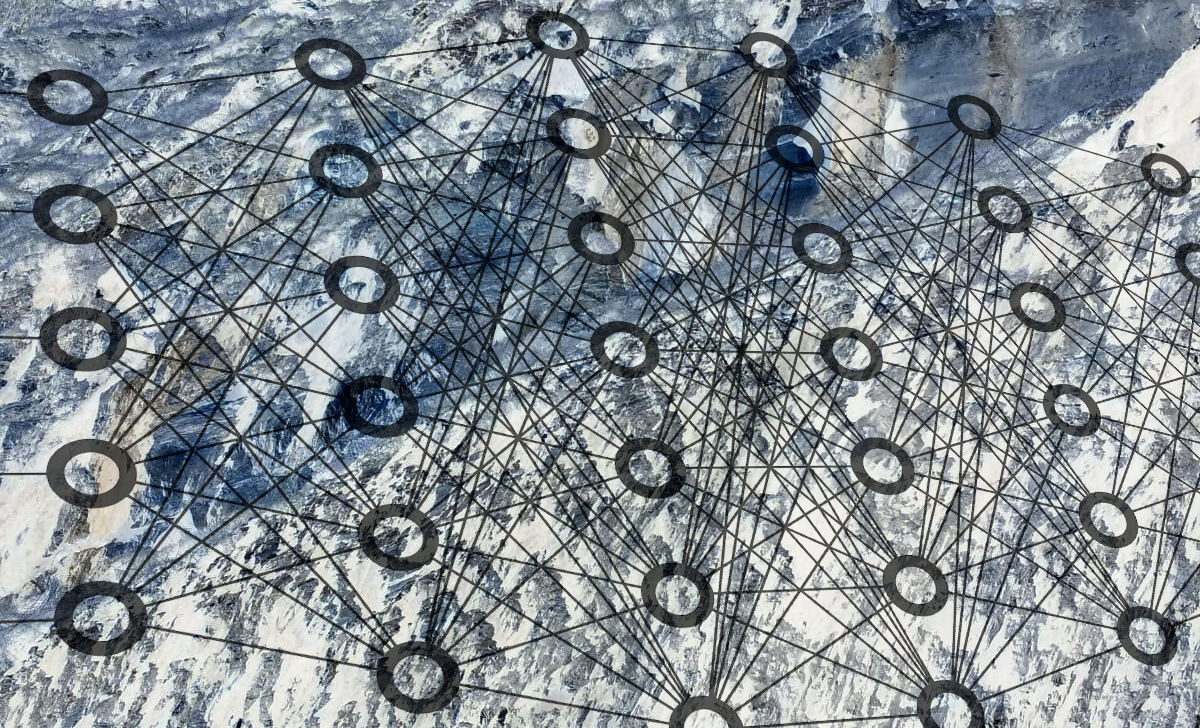
\includegraphics[height=\paperheight,width=\paperwidth]{frames/auxiliar/title_img/prueba.png}};}

\begin{frame}[plain]
\begin{variableblock}{}{bg=myblue,fg=white}{bg=green,fg=red}
\begin{center}
\textbf{1D Numerical results for Goal-Oriented $h$- and $p$-adaptivity}
\end{center}
\end{variableblock}
\end{frame}
}
%%%%%%%%%%%%%%%%%%%%%%%%%%%%%%%%%%%%%%%%%%%%%%%%%%%%%%%%%%%%%%%%%%%
\begin{frame}
  \frametitle{1D Numerical results for Goal-Oriented $h$- and $p$-adaptivity}
  \small % Reducing text size

  \begin{block}{Relative Error}
    The relative error in the Quantity of Interest (QoI) is defined as:
    \begin{equation}
      \scriptsize % Further reducing equation size
      e_{\textrm{rel}}^{\textrm{QoI}} \coloneqq \frac{|l(u) - l(u_{\mathcal{T}_{c}})|}{|l(u)|} \times 100,
    \end{equation}
    where $u$ is the fine grid solution, and $u_{\mathcal{T}_{c}}$ is the coarser mesh solution.
  \end{block} 
  
  \begin{block}{Helmholtz Goal-Oriented problem}
    Find $u$ such that:
    \begin{alignat}{2}
      \scriptsize % Reducing equation size
      -u'' -k^{2}u & = \mathds{1}_{(0,\frac{2}{5})} \quad \text{in} \ (0,1), \\
      u(0)         & = 0, \\
      u'(1)        & = 0.
    \end{alignat}
    QoI: $l(u)= 5 \int_{\frac{3}{5}}^{\frac{4}{5}} u \, dx$.
  \end{block}
\end{frame}

\begin{frame}
	\frametitle{Evolution of the Relative Error: $h$-adaptivity}
	\begin{figure}
  	\centering
  	\begin{tikzpicture}
    \begin{axis}[
        xlabel={DoF per wavelength},
        ylabel=Relative error in the QoI (\%),
        ymode=log,
        xmode=log,
        ylabel near ticks,
        xlabel near ticks,
        width=0.9\plotwidth,height=0.9\plotheight,
        legend style={draw=black, fill=white, legend cell align=left, at={(0.5,1.01)}, anchor=south},
        log x ticks with fixed point,
        xtick={3, 10, 40, 200, 600},
        legend columns=2,
      ]

      \addplot+[] table[x=DoFs_per_wavelength, y=Error]{Diapos/1d_numerical/Figures/Helm1D-7/h/order_1/outputs.txt}node[pos=0.61, pin={[pin edge=solid]180:$k=7 \cdot 2\pi$}]{};

      \addplot+[] table[x=DoFs_per_wavelength, y=Error]{Diapos/1d_numerical/Figures/Helm1D-14/h/order_1/outputs.txt}node[pos=0.8, pin={[pin edge=solid]-90:$k=14 \cdot 2\pi$}]{};

      \addplot+[] table[x=DoFs_per_wavelength, y=Error]{Diapos/1d_numerical/Figures/Helm1D-28/h/order_1/outputs.txt}node[pos=1, pin={[pin edge=solid]90:$k=28 \cdot 2\pi$}]{};

    \end{axis}
  \end{tikzpicture}
  	\caption{Evolution of $e_{\textrm{rel}}^{\textrm{QoI}}$ using $h$-adaptivity. Initial mesh size $h=\frac{1}{30}$ and uniform $p=1$.}
	\end{figure}	
\end{frame}

\begin{frame}
	\frametitle{Evolution of the Relative Error: $p$-adaptivity}
	\begin{figure}
  	\centering
  	\begin{tikzpicture}
    \begin{axis}[
        xlabel={DoF per wavelength},
        ylabel=Relative error in the QoI (\%),
        ymode=log,
        xmode=log,
        ylabel near ticks,
        xlabel near ticks,
        width=0.9\plotwidth,height=0.9\plotheight,
        legend style={draw=black, fill=white, legend cell align=left, at={(0.5,1.01)}, anchor=south},
        log x ticks with fixed point,
        xtick={4, 10, 20, 30},
        legend columns=2,
      ]

      \addplot+[] table[x=DoFs_per_wavelength, y=Error]{Diapos/1d_numerical/Figures/Helm1D-7/p/order_1/outputs.txt}node[pos=1, pin={[pin edge=solid] 180:$k=7 \cdot 2\pi$}]{};

      \addplot+[] table[x=DoFs_per_wavelength, y=Error]{Diapos/1d_numerical/Figures/Helm1D-14/p/order_1/outputs.txt}node[pos=0.75, pin={[pin edge=solid]180:$k=14 \cdot 2\pi$}]{};

      \addplot+[] table[x=DoFs_per_wavelength, y=Error]{Diapos/1d_numerical/Figures/Helm1D-28/p/order_1/outputs.txt}node[pos=0.65, pin={[pin edge=solid]180:$k=28 \cdot 2\pi$}]{};

    \end{axis}
  \end{tikzpicture}
  		\caption{Evolution of $e_{\textrm{rel}}^{\textrm{QoI}}$ using $p$-adaptivity. Uniform mesh size $h=\frac{1}{30}$.}
	\end{figure}	
\end{frame}

\begin{frame}
	\frametitle{Solution and Final Adaptive Meshes}
	\pgfplotsset{colormap/YlOrRd}

\begin{figure}
  \centering
  \begin{tikzpicture}[scale=0.85]
    \findmax{Diapos/1d_numerical/Figures/Helm1D-7/p/order_1/coarse_meshes/coarse_mesh_06.txt}{order}{\maxp}

    \begin{axis}[
        name=master,
        width=\textwidth,
        height=\plotheight,
        enlargelimits=false,
        enlarge y limits=true,
        enlarge y limits=0.15,
        xlabel=$x$,
        ylabel=$u(x)$,
      ]
      \addplot+[no markers, solid] table[x=X, y=My_beautiful_solution_real] {Diapos/1d_numerical/Figures/Helm1D-7/h/order_1/coarse_meshes/coarse_sol_dir_06.txt} node[pos=0.72, above]{direct};
      \addplot+[no markers, solid] table[x=X, y=My_beautiful_solution_real] {Diapos/1d_numerical/Figures/Helm1D-7/h/order_1/coarse_meshes/coarse_sol_adj_06.txt} node[pos=0.555, anchor=south west]{adjoint};
    \end{axis}

    \begin{axis}[
        name=pmesh,
        colormap access=const,
        colorbar horizontal,
        colorbar sampled,
        colorbar style={
          samples=\maxp+1,
          xtick={0.5,1.5,...,\maxp},
          xticklabels={1,2,...,\maxp},
          at={(master.above north west)},
          anchor=south west,
          title=Approximation order $p$,
          title style={yshift=3pt}, % Adjust the value as needed
          xticklabel pos=upper,
          yshift=1em,
          xtick style={draw=none},
          title style={yshift=2pt},
        },
        width=\textwidth,
        at={(master.south west)},
        enlargelimits=false,
        axis lines=none,
        height=2cm,
        ticks=none,
        point meta min=0,
        point meta max=\maxp,
        title=$p$-Mesh,
        title style={left, at={(0,0)}, align=right},
      ]
      \addplot [patch, patch type=rectangle, point meta=explicit, line width=0.1pt, faceted color=black] table[meta expr=\thisrow{order}-0.5] {Diapos/1d_numerical/Figures/Helm1D-7/p/order_1/coarse_meshes/coarse_mesh_06.txt};
    \end{axis}

    \begin{axis}[
        name=hmesh,
        width=\textwidth,
        at={(master.north west)},
        anchor=north west,
        enlargelimits=false,
        axis lines=none,
        height=2cm,
        ticks=none,
        point meta min=0,
        point meta max=\maxp,
        title=$h$-Mesh,
        title style={left, at={(0,0)}, align=right},
      ]
      \addplot [patch, patch type=rectangle, point meta=explicit, line width=0.1pt, faceted color=black] table[meta expr=\thisrow{order}-0.5] {Diapos/1d_numerical/Figures/Helm1D-7/h/order_1/coarse_meshes/coarse_mesh_05.txt};
    \end{axis}

  \end{tikzpicture}
  \caption{Solutions with $k = 7 \cdot 2 \pi$ problem after the $h$-adaptive process.}
\end{figure}
\end{frame}

\begin{frame}
  \frametitle{1D Numerical results for Goal-Oriented $h$- and $p$-adaptivity}
  \small % Reducing text size
  
  \begin{block}{Convection-diffusion Goal-Oriented problem}
   Find $u$ such that,
  \begin{alignat}{2}
    -\eps u'' + \sigma \cdot u' & = \mathds{1}_{\left(0,1\right)} &  & \text{ in } \left(0,1\right),\label{eq:convection} \\
    u\left(0\right)=u\left(1\right)                           & =0, \nonumber
  \end{alignat}
    The convection coefficient: $\sigma = 1$. \\
    The diffusive coefficient: $0 < \varepsilon \ll 1$. \\
    QoI: $l\left(u\right)=5 \cdot \int_{\frac{4}{5}}^{1} \grad u \, dx$.
  \end{block}
\end{frame}

\begin{frame}
	\frametitle{Evolution of the Relative Error: $h$-adaptivity}
	\begin{figure}
  	\centering
  \begin{tikzpicture}
    \begin{axis}[
        xlabel={nDoF},
        ylabel=Relative error in the QoI (\%),
        ymode=log,
        xmode=log,
        ylabel near ticks,
        xlabel near ticks,
        width=0.9\plotwidth,height=0.9\plotheight,
        legend style={draw=black, fill=white, legend cell align=left, at={(0.5,1.01)}, anchor=south},
        log x ticks with fixed point,
        xtick={30, 100, 400, 900},
        legend columns=2,
      ]

      \addplot+[] table[x=nr_dof, y=Error]{Diapos/1d_numerical/Figures/ConvDiff-eps3/h/order_1/outputs.txt}node[pos=0.61, pin={[pin edge=solid]180:$\eps= 10^{-3}$}]{};

      \addplot+[] table[x=nr_dof, y=Error]{Diapos/1d_numerical/Figures/ConvDiff-eps4/h/order_1/outputs.txt}node[pos=0.65, pin={[pin edge=solid]180:$\eps= 10^{-4}$}]{};

      \addplot+[] table[x=nr_dof, y=Error]{Diapos/1d_numerical/Figures/ConvDiff-eps5/h/order_1/outputs.txt}node[pos=0.61, pin={[pin edge=solid]180:$\eps= 10^{-5}$}]{};

    \end{axis}
  \end{tikzpicture}
  \caption{Evolution of $e_{\textrm{rel}}^{\textrm{QoI}}$ using $h$-adaptivity. Initial mesh size $h=\frac{1}{30}$ and uniform $p=1$.}
  \label{fig:error_qoi_h_ConvDiff}
\end{figure}
\end{frame}

\begin{frame}
	\frametitle{Evolution of the Relative Error: $p$-adaptivity}
	\begin{figure}
  	\centering
	\begin{tikzpicture}
    \begin{axis}[
        xlabel={nDoF},
        ylabel=Relative error in the QoI (\%),
        ymode=log,
        xmode=log,
        ylabel near ticks,
        xlabel near ticks,
        width=0.9\plotwidth,height=0.9\plotheight,
        legend style={draw=black, fill=white, legend cell align=left, at={(0.5,1.01)}, anchor=south},
        log x ticks with fixed point,
        xtick={30, 50, 100, 250, 450},
        legend columns=2,
      ]

      \addplot+[] table[x=nr_dof, y=Error]{Diapos/1d_numerical/Figures/ConvDiff-eps3/p/order_1/outputs.txt}node[pos=0.61, pin={[pin edge=solid]180:$\eps= 10^{-3}$}]{};

      \addplot+[] table[x=nr_dof, y=Error]{Diapos/1d_numerical/Figures/ConvDiff-eps4/p/order_1/outputs.txt}node[pos=0.61, pin={[pin edge=solid]180:$\eps= 10^{-4}$}]{};
      \addplot+[] table[x=nr_dof, y=Error]{Diapos/1d_numerical/Figures/ConvDiff-eps5/p/order_1/outputs.txt}node[pos=0.8, pin={[pin edge=solid]-90:$\eps= 10^{-5}$}]{};
    \end{axis}
  \end{tikzpicture}
  \caption{Evolution of $e_{\textrm{rel}}^{\textrm{QoI}}$ using $p$-adaptivity. Uniform mesh size $h=\frac{1}{30}$.}
  \label{fig:error_qoi_p_ConvDiff}
\end{figure}
\end{frame}

\begin{frame}
	\frametitle{Solution and Final Adaptive Meshes}
	\pgfplotsset{colormap/YlOrRd}

	\begin{figure}
  	\centering
	\begin{tikzpicture}[scale=0.85]
    \findmax{Diapos/1d_numerical/Figures/ConvDiff-eps3/p/order_1/coarse_meshes/coarse_mesh_08.txt}{order}{\maxp}

    \begin{axis}[
        name=master,
        width=\textwidth,
        height=\plotheight,
        enlargelimits=false,
        enlarge y limits=true,
        enlarge y limits=0.15,
        xlabel=$x$,
        ylabel=$u(x)$,
      ]
      \addplot+[no markers, solid] table[x=X, y=My_beautiful_solution_real] {Diapos/1d_numerical/Figures/ConvDiff-eps3/h/order_1/coarse_meshes/coarse_sol_dir_08.txt} node[pos=0.3, above, sloped]{direct};
      \addplot+[no markers, solid] table[x=X, y=My_beautiful_solution_real] {Diapos/1d_numerical/Figures/ConvDiff-eps3/h/order_1/coarse_meshes/coarse_sol_adj_08.txt} node[pos=0.8, above, sloped]{adjoint};
    \end{axis}

    \begin{axis}[
        name=pmesh,
        colormap access=const,
        colorbar horizontal,
        colorbar sampled,
        colorbar style={
          samples=\maxp+1,
          xtick={0.5,1.5,...,\maxp},
          xticklabels={1,2,...,\maxp},
          at={(master.above north west)},
          anchor=south west,
          title=Approximation order $p$,
          title style={yshift=3pt}, % Adjust the value as needed
          xticklabel pos=upper,
          yshift=1em,
          xtick style={draw=none},
          title style={yshift=2pt},
        },
        width=\textwidth,
        at={(master.south west)},
        enlargelimits=false,
        axis lines=none,
        height=2cm,
        ticks=none,
        point meta min=0,
        point meta max=\maxp,
        title=$p$-Mesh,
        title style={left, at={(0,0)}, align=right},
      ]
      \addplot [patch, patch type=rectangle, point meta=explicit, line width=0.1pt, faceted color=black] table[meta expr=\thisrow{order}-0.5] {Diapos/1d_numerical/Figures/ConvDiff-eps3/p/order_1/coarse_meshes/coarse_mesh_08.txt};
    \end{axis}

    \begin{axis}[
        name=hmesh,
        width=\textwidth,
        at={(master.north west)},
        anchor=north west,
        enlargelimits=false,
        axis lines=none,
        height=2cm,
        ticks=none,
        point meta min=0,
        point meta max=\maxp,
        title=$h$-Mesh,
        title style={left, at={(0,0)}, align=right},
      ]
      \addplot [patch, patch type=rectangle, point meta=explicit, line width=0.1pt, faceted color=black] table[meta expr=\thisrow{order}-0.5] {Diapos/1d_numerical/Figures/ConvDiff-eps3/h/order_1/coarse_meshes/coarse_mesh_08.txt};
    \end{axis}

  \end{tikzpicture}
  \caption{Solutions with $\eps=10^{-3}$ problem after the $h$-adaptive process.}
\end{figure}

\end{frame}
\end{section}
%%%%%%%%%%%%%%%%%%%%%%%%%%%%%%%%%%
%%%%%%%%%%%%%%%%%%%%%%%%%%%%%%%%%%
\begin{section}{2D Numerical results for $hp$-adaptivity}
%%%%%%%%
{
\usebackgroundtemplate{\tikz\node[opacity=0.1,inner sep=0] {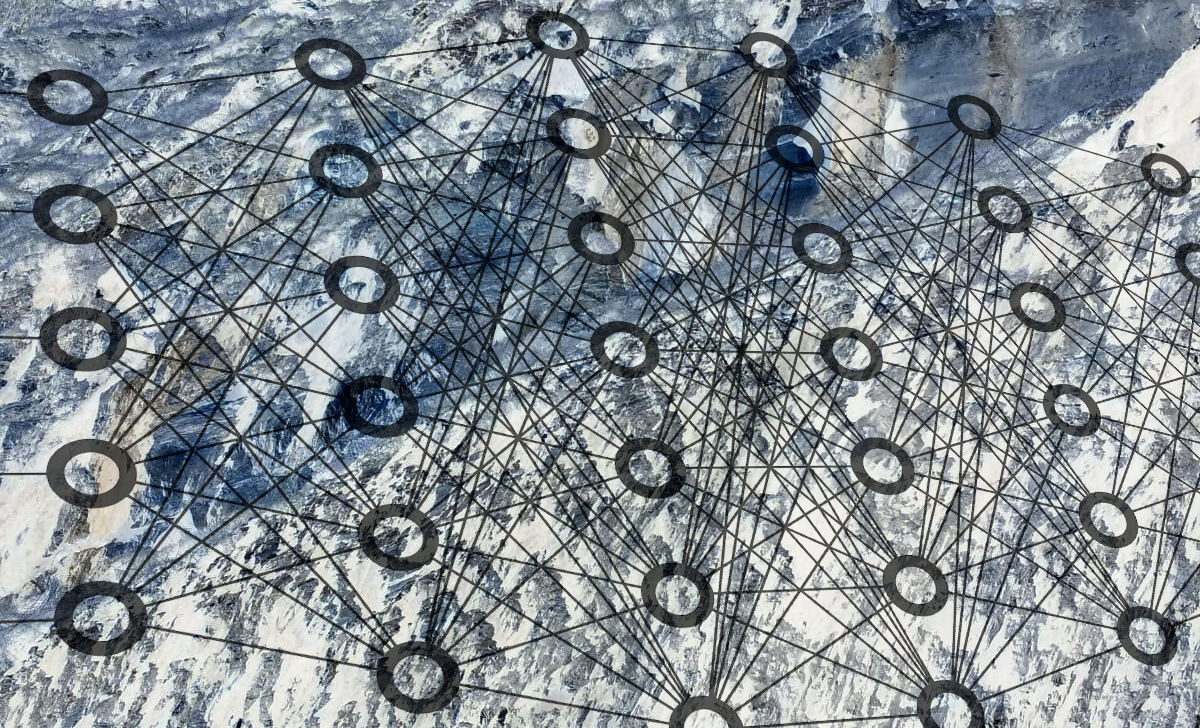
\includegraphics[height=\paperheight,width=\paperwidth]{frames/auxiliar/title_img/prueba.png}};}

\begin{frame}[plain]
\begin{variableblock}{}{bg=myblue,fg=white}{bg=green,fg=red}
\begin{center}
\textbf{2D Numerical results for $hp$-adaptivity}
\end{center}
\end{variableblock}
\end{frame}
}
%%%%%%%%%%%%%%%%%%%%%%%%%%%%%%%%%%%%%%%%%%%%%%%%%%%%%%%%%%%%%%%%%%%
\begin{frame}
  \frametitle{2D Numerical results for \( hp \)-adaptivity}

  \begin{block}{The relative error}
    In energy-norm adaptivity, we define the relative error in percentage as:
    \begin{equation}
	 \tilde{e}_{\textrm{rel}}^{\textrm{energy}} \coloneqq \frac{\norm{u - u_{\calT_{c}}}_{\H}}{\norm{u}_{\H}} \cdot 100.
    \end{equation}
  \end{block}
  
  \begin{block}{Our Quantity of Interest (QoI)}
    For the GOA problems, we define our QoI as
    \begin{equation}
      l\left(\phi\right) = 
      \frac{1}{\abs{\Omega_{l}}} \scalaire{\mathds{1}_{\Omega_{l}}}{\phi}_{L^2(\Omega)}, 
      \quad \forall \phi \in \H,
    \end{equation}
    where:
    \begin{itemize}
      \item \( \abs{\Omega_{l}} \) defines the area or volume of \( \Omega_{l} \),
      \item \( \mathds{1}_{\Omega_{l}} \) is a function equal to one if \( x \in \Omega_{l} \), and zero otherwise.
    \end{itemize}
  \end{block}

\end{frame}

\begin{frame}
  \frametitle{2D Numerical results for $hp$-adaptivity}

  \begin{block}{Singular Poisson example}
    Find \(u\) satisfying:
    \begin{alignat}{2}
      - \Delta u & = \mathds{1}_{\Omega_{f}} && \quad \text{in } \Omega, \\
      u          & = 0                       && \quad \text{on } \partial \Omega.
    \end{alignat}
  \end{block}

  \begin{multicols}{2}
   \textbf{Domain Definitions:}
    \begin{itemize}
      \item \(\Omega_{f} = \left(\frac{1}{4},\frac{1}{2}\right)^{2} \subset \Omega\), 
      \item \(\Omega_{l} = \left(\frac{1}{2},\frac{3}{4}\right)^{2} \subset \Omega\),
      \item \(a(\cdot ,\cdot) \coloneqq \scalar{\nabla \cdot}{\nabla \cdot}_{L^{2}(\Omega)}\).
    \end{itemize}
 
    \begin{figure}
       \centering
  	 \begin{tikzpicture}[x=3cm,y=3cm]
        % Nodes for regions
        \node (n1) at (0.25,0) {};
        \node (n2) at (0.75,0) {};
        \node (n3) at (0.75,0.25) {};
        \node (n4) at (0.25,0.25) {};
        \node (n5) at (0.5,0.5) {};
        \node (n7) at (0.75,0.75) {};

        % Rectangles and labels
        \draw (n4) rectangle (n5) node[pos=0.5] {\footnotesize $\Omega_{f}$};
        \draw (n5) rectangle (n7) node[pos=0.5] {\footnotesize $\Omega_{l}$};

        % Boundary and labels
        \draw[line width=0.5mm, color=blue] (0.25,0) -- (0.75,0) -- (0.75,0.25) -- (1,0.25) -- (1,0.75) -- (0.75,0.75) -- (0.75,1) -- (0.25,1) -- (0.25,0.75) -- (0,0.75) -- (0,0.25) -- (0.25,0.25) -- (0.25,0);
        \node at (0.5,0.9) {$\Omega$};

        % Labels at specific coordinates
        \node at (0,0) {$0$};
        \node at (1,0) {$1$};
        \node at (0,1) {$1$};

        % Dashed lines connecting labels
        \draw[dashed] (0.05,0) -- (0.97,0);
        \draw[dashed] (0,0.05) -- (0,0.96);
      \end{tikzpicture}
      \caption{Domain \\ $\Omega = \left(\left(0,1\right) \times \left(\frac{1}{4},\frac{3}{4}\right)\right) \cup \left(\left(\frac{1}{4},\frac{3}{4}\right) \times \left(0,1\right)\right)$.}
    \end{figure}
  \end{multicols}

\end{frame}

\begin{frame}
	\frametitle{Singular Poisson example}
	\begin{figure}[t!]
   		\goasolutions{CrossGOA}{real}
	\end{figure}
\end{frame}

\begin{frame}
	\frametitle{Singular Poisson example}
  	\plothpmeshes[]{CrossGOA}
\end{frame}

\begin{frame}
\frametitle{Singular Poisson Example}
\begin{figure}[t!]
\centering
\begin{tikzpicture}
\pgfplotsset{xmode=log, ymode=log} % Set log mode for both axes globally

\begin{axis}[
    name=mainerrorplot,
    xlabel={nDoFs (log scale)},
    ylabel={Relative error in \% (log scale)},
    ymode=log,
    xmode=log,
    width=0.9\plotwidth,
    height=0.9\plotheight,
    ylabel near ticks,
    xlabel near ticks,
    enlargelimits=true,
    legend style={
        draw=black,
        fill=white,
        legend cell align=left,
        at={(0.5,1.03)}, 
        anchor=south
    },
    legend columns=-1
]

% Plot for hp
\addplot+[line width=1pt] table[x expr=\thisrow{nr_dof}, y expr=\thisrow{Error}] {\FigurePath/CrossGOA/hp/order_1/outputs.txt}
    node[pos=0.85, pin={[pin edge=solid, pin distance=0.05cm]180:$hp$}] {}; % Adjusted pos from 0.9 to 0.85

% Plot for h with p=1
\addplot+[line width=1pt] table[x expr=\thisrow{nr_dof}, y expr=\thisrow{Error}] {\FigurePath/CrossGOA/h/order_1/outputs.txt}
    node[pos=0.9, pin={[pin edge=solid, pin distance=0.005cm]90:$h$ ($p=1$)}] {};

% Plot for h with p=2
\addplot+[line width=1pt] table[x expr=\thisrow{nr_dof}, y expr=\thisrow{Error}] {\FigurePath/CrossGOA/h/order_2/outputs.txt} 
    node[pos=1.010, pin={[pin edge=solid, pin distance=0.005cm]90:$h$ ($p=2$)}] {};

\end{axis}
\end{tikzpicture}
\caption{Evolution of $e_{\textrm{rel}}^{\textrm{QoI}}$ in the adaptive process.}
\end{figure}
\end{frame}

\end{section}
%%%%%%%%%%%%%%%%%%%%%%%%%%%%%%%%%%
%%%%%%%%%%%%%%%%%%%%%%%%%%%%%%%%%%
\begin{section}{Main Achievements}
{
\usebackgroundtemplate{\tikz\node[opacity=0.1,inner sep=0] {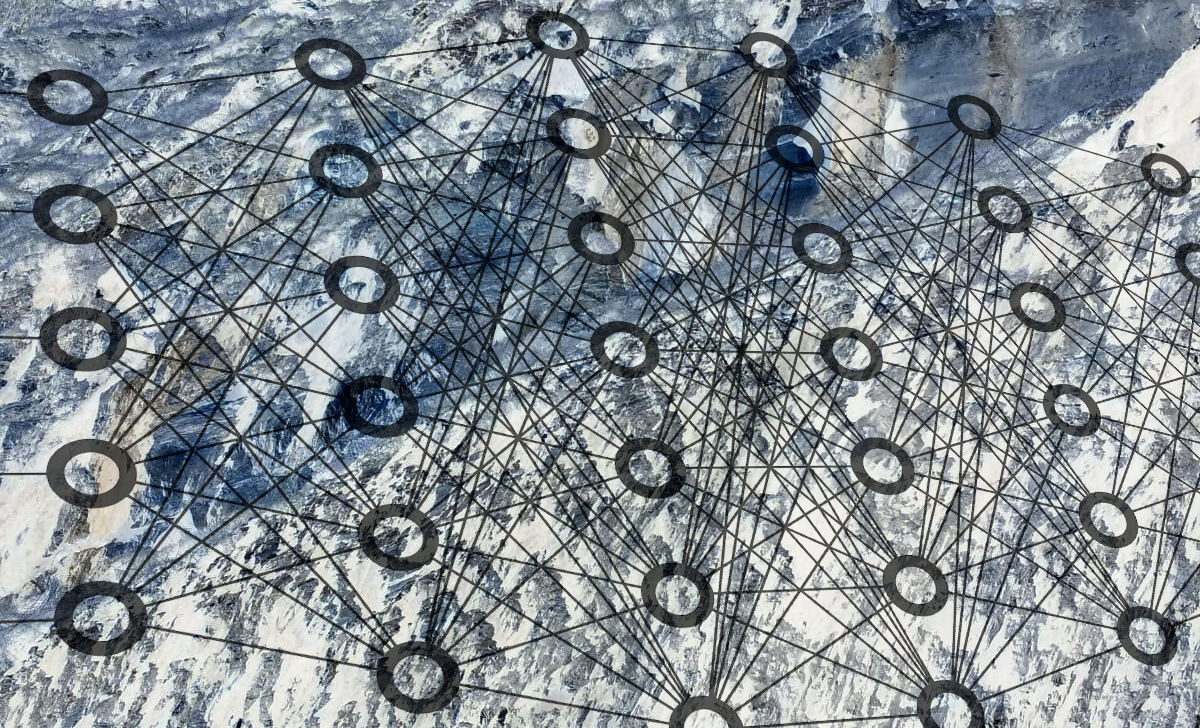
\includegraphics[height=\paperheight,width=\paperwidth]{frames/auxiliar/title_img/prueba.png}};}
%%%%%%%%
\begin{frame}[plain]

\begin{variableblock}{}{bg=myblue,fg=white}{bg=green,fg=red}
\begin{center}
\textbf{Main Achievements}
\end{center}
\end{variableblock}

\end{frame}
%%%%%%%%%%%%%%%%%%%%%%%%%%%%%%%%%%%%%%%%%%%%%%%%%%%%%%%%%%%%%%%%%%%
}
\begin{frame}{Main Achievements}
\textbf{Peer-Reviewed Publications}
\begin{thebibliography}{2}
\bibitem{mago}
{\small F. V. Caro, V. Darrigrand, J. Alvarez-Aramberri, and D. Pardo. ``A Multi-Adaptive-Goal-Oriented Strategy to Generate Massive Databases of Parametric PDEs,'' To be submitted to \textit{Computer Methods in Applied Mechanics and Engineering}, December 2023.}

\bibitem{painless}
{\small F. V. Caro, V. Darrigrand, J. Alvarez-Aramberri, E. Alberdi, and D. Pardo. ``A Painless Multi-Level Automatic Goal-Oriented $hp$-Adaptive Coarsening Strategy for Elliptic and Non-Elliptic Problems,'' \textit{Computer Methods in Applied Mechanics and Engineering}, vol. 401, 115641, 2022. \url{https://doi.org/10.1016/j.cma.2022.115641}}

\bibitem{ICCS}
{\small F. V. Caro, V. Darrigrand, J. Alvarez-Aramberri, E. A. Celaya, and D. Pardo. ``1D Painless Multi-Level Automatic Goal-Oriented $h$ and $p$ Adaptive Strategies Using a Pseudo-Dual Operator,'' In \textit{Computational Science -- ICCS 2022}, pp. 347--357, 2022. \url{https://doi.org/10.1007/978-3-031-08754-7_43}}
\end{thebibliography}
\end{frame}

\begin{frame}{Main Achievements}
\textbf{Conference Talks}
\vspace{0.2cm}

\begin{small}
\begin{tabular}{rl}
[1]& \underline{F. V. Caro}, V. Darrigrand, J. Alvarez-Aramberri, and D. Pardo. \\
& \textit{Databases for Deep Learning Inversion Using A Goal-Oriented $hp$-Adaptive Strategy.} \\
& XI International Conference on Adaptive Modeling and Simulation, \\
& Gothenburg, Sweden, June 19-21, 2023. \\\\
\end{tabular}

\begin{tabular}{rl}
[2]& \underline{F. V. Caro}, V. Darrigrand, J. Alvarez-Aramberri, E. Alberdi, and D. Pardo. \\
& \textit{A Painless Automatic $hp$-Adaptive Coarsening Strategy For Non-SPD problems:} \\
& \textit{A Goal-Oriented Approach.} 15th World Congress on Computational Mechanics \\
& \& 8th Asian Pacific Congress on Computational Mechanics, \\
& Yokohama, Japan, July 31 - August 5, 2022. \\\\
\end{tabular}

\begin{tabular}{rl}
[3]& \underline{F. V. Caro}, V. Darrigrand, J. Alvarez-Aramberri, E. Alberdi, and D. Pardo. \\
& \textit{1D Painless Multi-Level Automatic Goal-Oriented h and p Adaptive Strategies using} \\
& \textit{a Pseudo-Dual Operator.} 22nd International Conference on Computational Science, \\
& London, United Kingdom, June 21-23, 2022. \\\\
\end{tabular}
\end{small}

\end{frame}

\begin{frame}{Main Achievements}
\textbf{Conference Talks}
\vspace{0.2cm}

\begin{small}
\begin{tabular}{rl}
[4]&\underline{F. V. Caro}, V. Darrigrand, J. Alvarez-Aramberri, E. Alberdi, and D. Pardo. \\
& \textit{Goal-Oriented $hp$-Adaptive Finite Element Methods: A Painless Multilevel Automatic} \\
& \textit{Coarsening Strategy For Non-SPD Problems.} 8th European Congress on Computational \\
& Methods in Applied Sciences and Engineering, Oslo, Norway, June 5-9, 2022. \\\\
\end{tabular}

\begin{tabular}{rl}
[5]&\underline{F. V. Caro}, V. Darrigrand, J. Alvarez-Aramberri, E. Alberdi, and D. Pardo. \\
& \textit{A Painless Goal-Oriented $hp$-Adaptive Strategy for Indefinite Problems.} \\
& 16th U.S. National Congress on Computational Mechanics, \\
& Chicago, U.S.A, July 25-29, 2021. \\\\
\end{tabular}

\begin{tabular}{rl}
[6]&\underline{F. V. Caro}, V. Darrigrand, J. Alvarez-Aramberri, E. Alberdi, and D. Pardo. \\
& \textit{Goal-Oriented $hp$-Adaptive Finite Element Methods: A Painless Multi-level Automatic} \\
& \textit{Coarsening Strategy.} 10th International Conference on Adaptive Modeling and Simulation, \\
& Gothenburg, Sweden, June 21-23, 2021. \\\\
\end{tabular}
\end{small}

\end{frame}

\begin{frame}{Main Achievements}
\textbf{Research Stays}
\vspace{0.3cm}

\begin{small}
\begin{tabular}{rl}  
\textsc{Feb.} 2023 -- \textsc{Mar.} 2023 &University of Science and Technology (AGH),  \\
(2 months)& Krakow (Poland). \\
&\textbf{Supervisor:} Maciej Paszynski.\\
\end{tabular}
\vspace{0.5cm} % Add space here

\begin{tabular}{rl}  
\textsc{Sep.} 2021 -- \textsc{Nov.} 2021&CNRS-IRIT-ENSEEIHT (N7),  \\
(2 months)& Toulouse (France). \\
&\textbf{Supervisor:} Vincent Darrigrand.\\
\end{tabular}
\vspace{0.5cm} % And here

\begin{tabular}{rl}  
\textsc{Nov.} 2020 -- \textsc{Dec.} 2020&CNRS-IRIT-ENSEEIHT (N7),  \\
(1 month)& Toulouse (France). \\
&\textbf{Supervisor:} Vincent Darrigrand.\\
\end{tabular}
\end{small}

\end{frame}
%%%%%%%%%%%%%%%%%%%%%%%%%%%%%%%%%%%%%%%%%%%%%%%%%%%%%%%%%%%%%%%%%%%

%%%%%%%%%%%%%%%%%%%%%%%%%%%%%%%%%%%%%%%%%%%%%%%%%%%%%%%%%%%%%%%%%%%
\begin{frame}{Main Achievements}

\vspace{-1cm}
\begin{figure}
\begin{tikzpicture}

%comment the lint to show the image with a grid to help in finding the coordinates for the path.
\tikzset{develop clipping path=false}
\node at (5,0){
\clippicture{[width=5.2cm]{Diapos/Conclusions/img/bil_1.jpg}}{(0,0.5).. controls (0.2,1.15) and (0.8,1.15).. (1,0.5)-- (0.8,0)--(0.2,0)}
};


\tikzset{develop clipping path=false}
\node at (1,0){
\clippicture{[width=4.4cm]{Diapos/Conclusions/img/tls_1.jpg}}{(0,0.5).. controls (0.2,1.15) and (0.8,1.15).. (1,0.5)-- (0.8,0)--(0.2,0)}
};
\node at (2.5,2){Bilbao};
\node at (-1,-2){Toulouse};
\node at (10.5,-0.5){Kraków};

\node at (1,-3){
\clippicture{[height=2.2cm]{Diapos/Conclusions/img/tls_2.png}}{(0,0.5).. controls (0.2,1.15) and (0.8,1.15).. (1,0.5)-- (0.8,0)--(0.2,0)}
};

\node at (8,-2){
\clippicture{[height=3.5cm]{Diapos/Conclusions/img/agh_2.jpg}}{(0,0.5).. controls (0.2,1.15) and (0.8,1.15).. (1,0.5)-- (0.8,0)--(0.2,0)}
};

\node at (9,2){
\clippicture{[width=5cm]{Diapos/Conclusions/img/agh_1.jpg}}{(0,0.5).. controls (0.2,1.15) and (0.8,1.15).. (1,0.5)-- (0.8,0)--(0.2,0)}
};

%\node at (8,-4.3){Contact: \href{dzubiaur@gmail.com}{dzubiaur@gmail.com}};

%\draw[very thin,rounded corners=2pt, fill=orange!30!white ] (3,1) rectangle (7,2.5);
%\node[color=black] at (5,1.75) {\footnotesize \textcolor{black}{\textbf{\begin{tabular}{c} Research Stays \end{tabular}}}};

\end{tikzpicture}
\end{figure}

\end{frame}
%%%%%%%%%%%%%%%%%%%%%%%%%%%%%%%%%%%%%%%%%%%%%%%%%%%%%%%%%%%%%%%%%%%




\end{section}
%%%%%%%%%%%%%%%%%%%%%%%%%%%%%%%%%%
%%%%%%%%%%%%%%%%%%%%%%%%%%%%%%%%%%
\begin{section}{Conclusions and Future Work}
{
\usebackgroundtemplate{\tikz\node[opacity=0.1,inner sep=0] {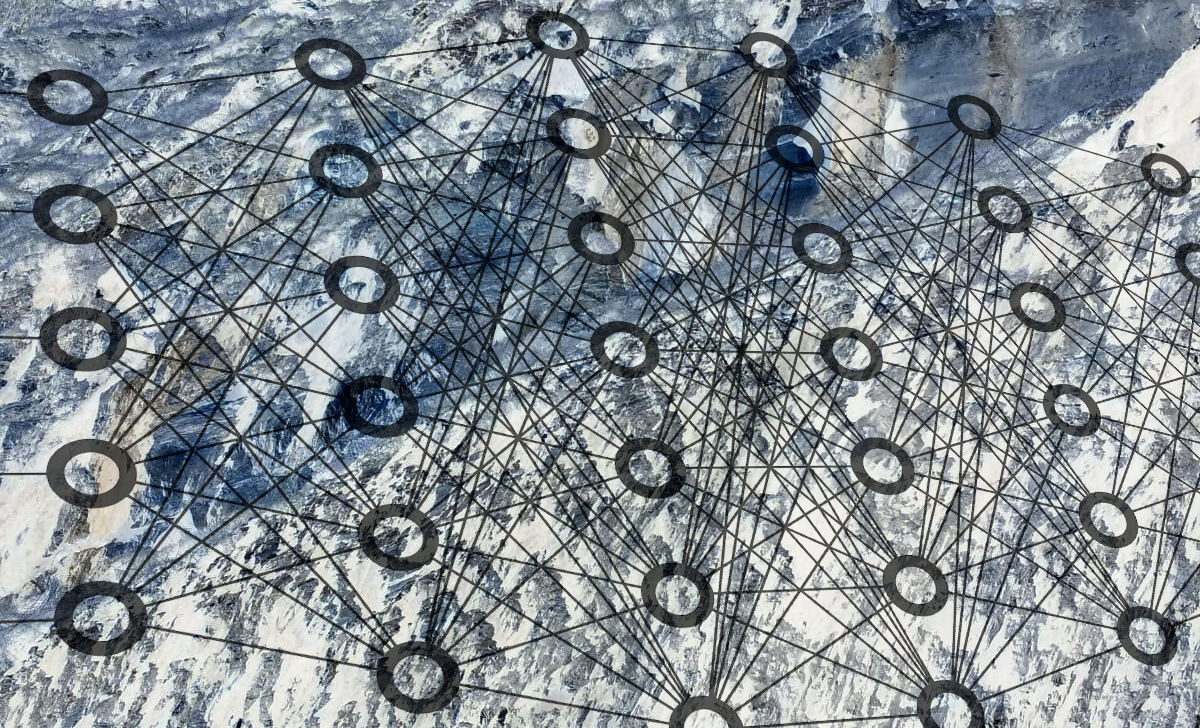
\includegraphics[height=\paperheight,width=\paperwidth]{frames/auxiliar/title_img/prueba.png}};}
%%%%%%%%
\begin{frame}[plain]

\begin{variableblock}{}{bg=myblue,fg=white}{bg=green,fg=red}
\begin{center}
\textbf{Conclusions and Future Work}
\end{center}
\end{variableblock}

\end{frame}
%%%%%%%%%%%%%%%%%%%%%%%%%%%%%%%%%%%%%%%%%%%%%%%%%%%%%%%%%%%%%%%%%%%
}
%%%%%%%%%%%%%%%%%%%%%%%%%%%%%%%%%%%%%%%%%%%%%%%%%%%%%%%%%%%%%%%%%%%
%%%%%%%%%%%%%%%%%%%%%%%%%%%%%%%%%%%%%%%%%%%%%%%%%%%%%%%%%%%%%%%%%%%
\begin{frame}{Contributions}

\begin{itemize}
\item We have employed hierarchical basis functions that effectively address the challenge of \emph{hanging nodes}.
\vspace{0.3cm}
\item We have developed \textbf{simple-to-implement} \( h \)- and \( p \)-GOA strategies that use an unconventional symmetric and positive definite bilinear form for possibly non-elliptic goal-oriented problems.
\vspace{0.3cm}
\item We have expanded upon a painless automatic \( hp \) strategy, initially developed for energy-norm adaptivity, to both non-elliptic and goal-oriented problems.
\vspace{0.3cm}
\item We have extended the applicability of a coarsening strategy to encompass parametric PDEs.
\vspace{0.3cm}
\end{itemize}

\end{frame}
%%%%%%%%%%%%%%%%%%%%%%%%%%%%%%%%%%%%%%%%%%%%%%%%%%%%%%%%%%%%%%%%%%%

%%%%%%%%%%%%%%%%%%%%%%%%%%%%%%%%%%%%%%%%%%%%%%%%%%%%%%%%%%%%%%%%%%%
%%%%%%%%%%%%%%%%%%%%%%%%%%%%%%%%%%%%%%%%%%%%%%%%%%%%%%%%%%%%%%%%%%%
\begin{frame}{Future Work}

\begin{itemize}
\item Reduce data needed to perform inversion using DL.
\vspace{0.5cm}
\item Implement adaptive integration methods in higher dimensions.
\vspace{0.5cm}
\item Develop $r$-adaptive methods to improve piecewise-polynomial approximation.
\vspace{0.5cm}
\item Solve parametric PDEs using NNs.
\end{itemize}

\end{frame}
%%%%%%%%%%%%%%%%%%%%%%%%%%%%%%%%%%%%%%%%%%%%%%%%%%%%%%%%%%%%%%%%%%%

\end{section}

\end{document}